%% KALAVAI: Cooperative LLM Training via Independent Specialists
%% NeurIPS 2026 Submission -- Double-blind anonymous version
%%
%% To compile:
%%   pdflatex kalavai_neurips2026_submit.tex
%%   bibtex kalavai_neurips2026_submit
%%   pdflatex kalavai_neurips2026_submit.tex
%%   pdflatex kalavai_neurips2026_submit.tex
%%
%% Requires: neurips_2026.sty (included in this directory)

\documentclass{article}

\usepackage{neurips_2026}  % Default = anonymous double-blind submission with line numbers

\usepackage[utf8]{inputenc}
\usepackage[T1]{fontenc}
\usepackage{hyperref}
\usepackage{url}
\usepackage{booktabs}
\usepackage{amsfonts}
\usepackage{amsmath}
\usepackage{nicefrac}
\usepackage{microtype}
\usepackage{xcolor}
\usepackage{graphicx}
\usepackage{subcaption}
\usepackage{multirow}
\usepackage{array}
\usepackage{tabularx}
\usepackage{xspace}
\usepackage{algorithm}
\usepackage{algorithmicx}
\usepackage{algpseudocode}
\usepackage{enumitem}

\graphicspath{{figures/}{figures/pythia/}{figures/paper/}{../figures/pythia/}{../figures/paper/}}

% Convenience macros
\newcommand{\kalavai}{\textsc{Kalavai}\xspace}
% Tamil script (kalaVAI / \u0B95\u0BB2\u0BB5\u0BC8) cannot be rendered in pdflatex without a Tamil Type1 font.
% arXiv requires pdflatex, so we use the ISO 15919 romanisation with a note.
\newcommand{\tamil}{\textit{kalaVAI}\xspace}
\newcommand{\eg}{\emph{e.g.}\xspace}
\newcommand{\ie}{\emph{i.e.}\xspace}
\newcommand{\cf}{\emph{cf.}\xspace}
\newcommand{\etal}{\emph{et al.}\xspace}
\newcommand{\todo}[1]{\textcolor{red}{[TODO: #1]}}

\title{KALAVAI: Predicting When Independent Specialist Fusion Works\\
       A Quantitative Model for Post-Hoc Cooperative LLM Training}

\author{%
  Anonymous Authors
}

\begin{document}

\maketitle

\begin{abstract}
Independently trained domain specialists can be fused post-hoc into a single model that outperforms any individual specialist---and the gain is predictable before training begins:
$\text{gain} \approx 0.82 \times \text{divergence} - 2.72$ ($R^2 = 0.856$, $n=6$, spanning 3--26\% divergence).
A cooperative whose specialists diverge 15\% from the shared base checkpoint yields approximately $+7.5\%$ improvement over the best individual specialist.
Below $\approx$3.3\% divergence the formula predicts near-zero gain; practitioners can verify specialist divergence before committing training resources.

In the \kalavai\footnote{KALAVAI (\textit{kalaVAI}) is the ISO~15919 romanisation of the Tamil word for ``fusion'' or ``mixing''.} protocol, contributors each fine-tune a copy of a shared base checkpoint on their own data without communication, then submit checkpoints for lightweight MoE routing (500 gradient steps on mixed data).
Gains are consistent across scales: $+7.72\%$ at 410M ($\pm$0.02\%, 3 seeds), $+7.49\%$ at 1B ($\pm$0.01\%, 3 seeds), and $+6.53\%$ at 6.9B, each over the best individual specialist.
The fused model achieves oracle-optimal routing: the learned router matches the domain oracle with gap $<10^{-5}$ nats.
Phase 2 extends the protocol to high-divergence settings: cross-lingual fusion (Tamil/Yoruba/Welsh/Code) achieves $+21.76\%$, with Yoruba perplexity falling $41.9\to7.7$.
A 20-contributor federation (10 languages + 10 domains) achieves $+16.71\%$ ($\pm$0.07pp, 3 seeds) vs.\ best specialist.

Three structural requirements bound the protocol. \emph{Shared initialisation} is necessary: specialists from mismatched checkpoints degrade routing clarity. \emph{Frozen layers} are optional below approximately 10,000 specialist training steps---peak gain reaches $+17.7\%$ at 5,000 steps without freezing---and become beneficial at longer training horizons. \emph{Learned routing} is essential: uniform equal-weight averaging degrades by $-1.2\%$ versus the best specialist, while a trained linear or MLP router achieves oracle-optimal assignment; routing architecture has minimal effect once gates are trained.
\end{abstract}

% ============================================================
\section{Introduction}
\label{sec:intro}
% ============================================================

Training competitive language models requires centralised compute at a scale most researchers and institutions cannot access. A single 70B-parameter training run requires hundreds of A100 GPUs operating synchronously for weeks. This creates a structural barrier: the organisations that can train frontier models are those that can pay for frontier compute, and the rest must fine-tune what is already available.

\paragraph{The core insight.} A different path exists. If multiple contributors each train a \emph{specialist} copy of a shared base checkpoint on their own domain, and if those specialists are subsequently fused via a learned router, the resulting model captures complementary knowledge that no single contributor could build alone. The training step requires no communication: contributors work independently, asynchronously, on their own hardware, using their own data. The only coordination is the shared starting point. The fused model requires all $N$ specialists to run at inference, increasing inference compute by a factor of $N$ relative to any individual specialist. This is a training-time democratisation: inference cost scales with $N$ specialists, but so does the knowledge that no single contributor could acquire alone.

This observation is not entirely new---the branch-train-mix (BTX) paradigm \citep{sukhbaatar2024branchtrainmix} demonstrates that MoE fusion of independently trained models is feasible. What is missing from the literature is an empirical characterisation of \emph{the conditions under which independent specialist fusion succeeds or fails}: when shared initialisation alone is sufficient, when frozen layers become necessary, and what routing architecture drives improvement.

\paragraph{The protocol.} \kalavai operationalises cooperative LLM training as a four-step protocol: (1) a coordinator distributes a shared base checkpoint; (2) each contributor fine-tunes independently on their domain for a fixed number of steps; (3) contributors submit their checkpoints; (4) a lightweight router is trained on a small mixed-domain dataset and used for inference. Contributors never share gradients, intermediate activations, or data. The only shared artefact is the initial checkpoint.

\paragraph{Key results.} We validate the protocol across six experimental conditions spanning 3--26\% specialist divergence. Fusion gain scales linearly with divergence ($\text{gain} = 0.82 \times \text{div} - 2.72$, $R^2 = 0.856$, $n=6$), enabling practitioners to estimate cooperative value before training. At three scales, \kalavai consistently outperforms the best individual specialist: $+7.72\%$ at 410M ($\pm$0.02\%, 3 seeds), $+7.49\%$ at 1B ($\pm$0.01\%, 3 seeds), and $+6.53\%$ at 6.9B. Routing must be trained---uniform mixing degrades by $-1.19\%$ while a simple linear router achieves oracle-optimal assignment---but routing architecture is otherwise unimportant. Phase 2 extends the protocol to private professional domains ($+10.17\%$), cross-lingual settings ($+21.76\%$, Yoruba PPL $41.9\to7.7$), and a 20-contributor federation ($+16.71\%$, $\pm$0.07pp, 3 seeds). Our contributions are a predictive divergence--gain formula, an empirical characterisation of when fusion succeeds or fails, and practitioner guidelines for cooperative LLM training. Code, scripts, and result artefacts are released publicly.\footnote{All results use the per-domain equal-weight protocol; see Appendix~\ref{app:evalcorrection}.}

% ============================================================
\section{Related Work}
\label{sec:related}
% ============================================================

\paragraph{Branch-Train-Mix (BTX).} The closest prior work is BTX \citep{sukhbaatar2024branchtrainmix}, which demonstrates that models branched from a shared checkpoint, independently trained, and mixed via MoE routing form a better model than any individual branch. Building on this foundation, our empirical contribution addresses four questions that remain open in the literature: when shared initialisation alone is sufficient versus when frozen layers become necessary (Section~\ref{sec:crossover}); whether improvement persists against a compute-matched monolithic baseline (Section~\ref{sec:monolithic}); when routing must be trained versus when uniform routing suffices (Section~\ref{sec:failure}); and whether improvement is explained by increased parameter count (Section~\ref{sec:capacity}). BTX demonstrates fusion at comparable model scales with substantially longer specialist training budgets; our focus is the systematic conditions analysis rather than a head-to-head performance comparison.

\paragraph{MoErging and PHATGOOSE.} The MoErging survey \citep{yadav2024merging} taxonomises approaches for recycling and routing among independently trained experts. PHATGOOSE \citep{muqeeth2024phatgoose} achieves +11\% zero-shot generalisation improvement via learned routing among fine-tuned models, compared to \kalavai's $+7.72\%$ vs.\ best-specialist or +16.3\% vs.\ base on held-out evaluation. \kalavai adds a monolithic baseline, training duration analysis, and explicit capacity controls not present in PHATGOOSE.

\paragraph{Pari thesis.} \citet{pari2025merging} provides a theoretical analysis using Centered Kernel Alignment (CKA) of why weight averaging of independently trained models fails: divergent representations produce destructive interference when merged by linear interpolation. \kalavai provides the empirical complement, demonstrating that MoE routing avoids this interference (+7.72\% vs.\ best specialist versus weight averaging's $-$3.4\% vs.\ best specialist).

\paragraph{Weight interpolation methods.} Model soups \citep{wortsman2022modelsoups}, TIES-Merging \citep{yadav2023tiesmerging}, and DARE \citep{yu2023dare} combine fine-tuned models via weight interpolation. These methods require specialised merging procedures and typically produce smaller gains than routing-based approaches. In our experiments, simple weight averaging achieves $-$3.4\% vs.\ best specialist (equal-weight evaluation) versus +7.72\% for learned MoE routing.

\paragraph{Other related approaches.} Federated learning requires gradient synchronisation \citep{mcmahan2017federated}; FuseLLM uses knowledge distillation \citep{wan2024fusellm}; sparse upcycling initialises MoE from dense checkpoints \citep{komatsuzaki2023sparseupcycling}; STAR demonstrates modular composition \citep{qin2025star}. None provides the conditions analysis we contribute. Extending specialist fusion to low-resource languages (Section~\ref{sec:phase2}) has not been studied in prior work.

% ============================================================
\section{Method}
\label{sec:method}
% ============================================================

The \kalavai protocol consists of four phases.

\paragraph{Phase 1: Shared initialisation.} A coordinator selects a publicly available base checkpoint $\theta_0$ and distributes it to all contributors. All specialists begin from \emph{identical} weights. This shared initialisation is the core structural guarantee that enables post-hoc fusion: specialists diverge in representation space, but their representational geometry remains compatible because they begin from the same point. Hash verification ensures all contributors use exactly the same checkpoint.

\paragraph{Phase 2: Optional freezing.} Optionally, the first $K$ transformer layers are frozen during specialist training. Frozen layers guarantee that lower-level representations remain shared across specialists, providing a structural anchor that is robust to extended training. Our experiments show freezing is unnecessary at short training horizons ($\leq$10,000 steps) but becomes beneficial beyond approximately 10,000 steps (Section~\ref{sec:crossover}).

\paragraph{Phase 3: Independent specialist training.} Each contributor trains their copy of $\theta_0$ on a single knowledge domain using standard next-token prediction loss. Training is fully independent: contributors never share data, gradients, or activations. Any training infrastructure, hardware, or optimiser the contributor prefers may be used, provided the architecture and freeze configuration match the coordinator's specification. We use full fine-tuning of unfrozen layers; LoRA fails to produce useful divergence (Appendix~\ref{app:design}).

Formally, contributor $i$ trains specialist $\theta_i$ by minimising:
\[
\mathcal{L}_i = -\mathbb{E}_{x \sim \mathcal{D}_i} \left[\sum_t \log p_{\theta_i}(x_t \mid x_{<t})\right]
\]
where $\mathcal{D}_i$ is contributor $i$'s domain-specific dataset and $\theta_i$ shares the first $K$ frozen layers with all other specialists.

\paragraph{Phase 4: Post-hoc MoE fusion.} After all specialists submit their checkpoints, a lightweight router is trained on a small mixed-domain dataset (500 gradient steps in our experiments). The router is a single linear layer mapping the model's hidden state at position $t$ to a distribution over experts:
\[
g_t = \mathrm{softmax}\left(W_r \cdot h_t\right), \quad W_r \in \mathbb{R}^{N \times d}
\]
where $h_t$ is the mean-pooled final hidden state averaged across all specialists' forward passes (see Appendix~\ref{app:dynamics}), $N$ is the number of specialists, and $d$ is the hidden dimension. At inference, all $N$ specialists process each token in parallel and the fused output is a weighted combination of their \emph{logit vectors}:
\[
\tilde{l}_t = \sum_{i=1}^{N} g_t^{(i)} \cdot l_{\theta_i,t}, \qquad
p_\text{fused}(x_t \mid x_{<t}) = \mathrm{softmax}\!\left(\tilde{l}_t\right)
\]
where $l_{\theta_i,t} \in \mathbb{R}^{|\mathcal{V}|}$ is the logit vector from specialist $i$ at position $t$. This logit-space combination---equivalent to a log-linear mixture---is standard in MoE architectures~\citep{shazeer2017outrageously,jiang2024mixtral}.

Design choices are discussed in Appendix~\ref{app:design}; none meaningfully affects the core results.

% ============================================================
\section{Experiments}
\label{sec:experiments}
% ============================================================

\subsection{Experimental Setup}
\label{sec:setup}

\paragraph{Models.} We run experiments at three scales: Pythia-410M (24 layers, hidden size 1024), Pythia-1B (16 layers, hidden size 2048), and Pythia-6.9B (32 layers, hidden size 4096) \citep{biderman2023pythia}. All experiments initialise from the \texttt{step10000} Pythia checkpoint, which corresponds to 7\% of total pre-training. We use Pythia because it releases checkpoints at multiple training stages, enabling the maturity sweep analysis.

\paragraph{Domains.} Three domain specialists are trained per experiment: (1) \emph{code} (CodeSearchNet Python subset), (2) \emph{science} (SciQ with supporting context), and (3) \emph{fiction} (PG-19 books). For each domain, 90\% of samples are used for specialist training, 10\% are held out and never seen during training or router training.

\paragraph{Training configuration.} All 410M and 1B experiments: 2,000 specialist training steps (effective batch size 8, sequence length 512), 500 router training steps. 6.9B experiments: 1,000 specialist training steps, 500 router steps. Freeze depth $K=4$ for 410M (4/24 = 17\%), $K=4$ for 1B (4/16 = 25\%), $K=6$ for 6.9B (6/32 = 19\%). Optimiser: AdamW, $\text{lr}=2\times10^{-5}$, weight decay 0.1, linear warmup over 10\% of steps.

\paragraph{Evaluation metric.} All improvement percentages are computed as:
\[
\Delta(\%) = \frac{\mathcal{L}_\text{baseline} - \mathcal{L}_\text{method}}{\mathcal{L}_\text{baseline}} \times 100
\]
where $\mathcal{L}$ is average cross-entropy loss on the held-out mixed-domain evaluation set (equal weighting across three domains). Lower loss is better; positive $\Delta$ indicates improvement over the baseline. The baseline for the main result is the best individual specialist on mixed evaluation; the baseline for the monolithic comparison is the monolithic model.

\paragraph{Seeds.} All main results are reported across 3 random seeds (42, 137, 2026).

\paragraph{Evaluation.} All results use the per-domain equal-weight protocol (base EW loss 2.651 at 410M, bs=4): each domain evaluated separately at consistent batch size, equal-weight average.

\subsection{Core Results}
\label{sec:core}

\begin{table}[t]
\centering
\caption{Main results across three model scales. \textbf{Per-domain equal-weight evaluation}: each domain evaluated separately at bs=4; equal-weight average $= (\mathcal{L}_\text{code} + \mathcal{L}_\text{sci} + \mathcal{L}_\text{fiction})/3$ (Appendix~\ref{app:evalcorrection}). 410M results: 3-seed means (seeds 42/137/2026). 6.9B: seed 42. All results seed 42 or means over 3 seeds where noted.}
\label{tab:main}
\begin{tabular}{llcccccc}
\toprule
\textbf{Scale} & \textbf{Method} & \textbf{EW Loss} & \textbf{vs.\ Best Spec.} & \textbf{vs.\ Base} & \textbf{Seeds} & \textbf{Std} \\
\midrule
\multirow{5}{*}{Pythia-410M}
 & Base model          & 2.651 & ---     & ---     & ---  & ---       \\
 & Best specialist     & 2.404 & ---     & +9.3\%  & 3    & $\pm$0.02\% \\
 & Weight averaging    & 2.486 & $-$3.4\% & +6.2\% & 3    & $\pm$0.00\% \\
 & Monolithic baseline & 2.229 & ---     & +16.0\% & 3    & $\pm$0.00\% \\
 & \kalavai (MoE)      & \textbf{2.218} & \textbf{+7.72\%} & +16.3\% & 3 & $\pm$0.02\% \\
\midrule
\multirow{3}{*}{Pythia-1B}
 & Base model          & 2.474 & ---     & ---     & ---  & ---        \\
 & Best specialist     & 2.259 & ---     & +8.7\%  & 1    & ---        \\
 & Monolithic baseline & 2.097 & ---     & +15.3\% & 1    & ---        \\
 & \kalavai (MoE)      & \textbf{2.090} & \textbf{+7.49\%} & +15.5\% & 3 & $\pm$0.01\% \\
\midrule
\multirow{3}{*}{Pythia-6.9B}
 & Base model          & 2.320 & ---     & ---     & ---  & ---        \\
 & Best specialist     & 2.266 & ---     & +2.3\%  & 1    & ---        \\
 & \kalavai (MoE)      & \textbf{2.118} & \textbf{+6.53\%} & +8.7\%  & 3 & $\pm$0.024\% \\
\bottomrule
\end{tabular}
\end{table}

Table~\ref{tab:main} presents the main results under per-domain equal-weight evaluation. \kalavai consistently outperforms the best individual specialist at all tested scales. The 410M improvement of +7.72\% is robust: variance across three random seeds is near-zero ($\pm$0.02\%), and results are stable across Pythia training maturities (see Appendix~\ref{app:maturity}).

The 6.9B improvement (+6.53\%, $\pm$0.024\%, 3 seeds) is smaller than at 410M/1B, but the underlying mechanism is unchanged. At 410M and 1B, domain specialists diverge 10--25\% from the base (mean $\approx$15.5\%), yielding $\approx$+7.5\% fusion gain. At 6.9B, divergence is roughly half---7--10\% per domain (mean 8.73\%, Table~\ref{tab:divergence})---and the gain scales proportionally. Notably, \emph{conversion efficiency} (gain per unit divergence) is higher at 6.9B ($0.75\times$) than at 410M/1B ($0.49\times$): larger models translate divergence into fusion gain more effectively. The reduced absolute gain at 6.9B therefore reflects reduced specialist divergence, not scale-dependent degradation of the protocol. Routing is near-deterministic across all scales ($>$99.9\% per-domain gate weight), and improvement is stable across training maturities from 3.5\% to 100\% of pre-training (+7.0\%--+8.8\%; Appendix~\ref{app:maturity}).

\begin{table}[h]
\centering
\caption{Specialist divergence (per-domain improvement over base, \%) and fusion gain (MoE vs.\ best individual specialist, equal-weight), seed 42. Per-domain separate eval at consistent batch size (bs=4). $\dagger$~Qwen-1.5B uses code + fiction only (2 specialists). Fusion gain conversion rate = gain/divergence. All Pythia routing $>$99.9\% per-domain deterministic.}
\label{tab:divergence}
\small
\begin{tabular}{lcccccc}
\toprule
\textbf{Model} & \textbf{Code div.} & \textbf{Sci.\ div.} & \textbf{Fiction div.} & \textbf{Mean div.} & \textbf{Fusion gain} & \textbf{Conv.\ rate} \\
\midrule
Pythia-410M         & 9.97\%  & 11.60\% & 25.37\% & 15.65\% & +7.72\% & 0.49$\times$ \\
Pythia-1B           & 11.05\% & 9.39\%  & 25.41\% & 15.28\% & +7.49\% & 0.49$\times$ \\
Pythia-6.9B         & 9.28\%  & 10.16\% & 6.76\%  & 8.73\%  & +6.53\% & 0.75$\times$ \\
Qwen-1.5B$^\dagger$ & 1.76\%  & ---     & 4.56\%  & 3.16\%  & +1.06\% & 0.34$\times$ \\
\bottomrule
\end{tabular}
\end{table}

\paragraph{Evaluation protocol.} All reported improvements use the per-domain equal-weight protocol: each domain evaluated separately at bs=4, gains averaged equally across domains. Full specification and implementation details are in Appendix~\ref{app:evalcorrection}.

\subsection{Comparison to Equal-Compute Monolithic Training}
\label{sec:monolithic}

\begin{figure}[t]
  \centering
  \includegraphics[width=0.9\textwidth]{fig_hero_2panel}
  \caption{\textbf{\kalavai core results.} \textbf{(A)} Fusion improvement over the best individual specialist across model scales: $+7.72\%$ at 410M, $+7.49\%$ at 1B, $+6.53\%$ at 6.9B (per-domain equal-weight eval). Gains are proportional to specialist divergence; conversion rate $0.49\times$ at 410M/1B, $0.75\times$ at 6.9B. \textbf{(B)} Training duration crossover: freeze=0 peaks at 5k steps ($+17.7\%$) then degrades to $+14.7\%$ at 20k steps; freeze=4 degrades more slowly ($+17.0\%$ at 20k); crossover at $\approx$10k steps. Router architecture (panel C) and monolithic comparison (panel D) are in Appendix~\ref{app:herofull}. All results seed 42 or means over 3 seeds where noted.}
  \label{fig:hero}
\end{figure}

A natural question is whether centralised training on equivalent total compute would perform equally well. We test this directly at both 410M and 1B scales. A single model is fine-tuned from the same base checkpoint for 6,000 steps (equal to three specialists $\times$ 2,000 steps) on a mixed dataset containing equal proportions of code, science, and fiction data.

The monolithic baseline achieves strong results: 410M monolithic EW loss 2.229 (+16.0\% vs.\ base) vs.\ \kalavai MoE EW loss 2.218 (+0.47\% over monolithic, Table~\ref{tab:monolithic}). At 1B, monolithic EW loss 2.097 vs.\ \kalavai 2.090 (+0.34\% over monolithic). The cooperative MoE and equal-compute monolithic model achieve near-parity on this metric. The main headline result of \kalavai is the advantage over the \emph{best individual specialist}: +7.72\% at 410M (specialist EW loss 2.404 vs.\ MoE 2.218), driven by the router recovering each domain's specialist quality simultaneously.

\paragraph{Per-domain advantage.} The \kalavai MoE matches the best individual specialist on \emph{every domain simultaneously}: code loss 1.8791 (= code specialist), science 2.5565 (= science specialist), fiction 2.2194 (= fiction specialist). The oracle gap is $3\times10^{-6}$ nats---the learned router has converged to the domain-level optimum. The monolithic model underperforms the MoE on code ($-4.34\%$) and science ($-3.12\%$), showing that per-domain specialist quality is the cooperative advantage over centralised training (full breakdown in Appendix~\ref{app:monolithic}).

\begin{table}[h]
\centering
\caption{Equal-compute comparison at Pythia-410M and Pythia-1B. Monolithic trained for 6,000 steps on mixed data; \kalavai uses three specialists $\times$ 2,000 steps. Equal-weight per-domain average (per-domain separate eval, bs=4). Seed 42. The monolithic model achieves strong equal-weight loss because it trains on all domains; \kalavai's advantage is per-domain specialist quality for each domain simultaneously.}
\label{tab:monolithic}
\begin{tabular}{llccc}
\toprule
\textbf{Scale} & \textbf{Method} & \textbf{EW Loss} & \textbf{vs.\ Base} & \textbf{vs.\ Monolithic} \\
\midrule
\multirow{4}{*}{410M}
 & Base model            & 2.651 & ---      & ---       \\
 & Best specialist       & 2.404 & +9.3\%  & ---       \\
 & Monolithic (6k steps) & 2.229 & +16.0\% & ---       \\
 & \kalavai MoE          & \textbf{2.218} & +16.3\% & +0.47\% \\
\midrule
\multirow{4}{*}{1B}
 & Base model            & 2.474 & ---      & ---       \\
 & Best specialist       & 2.259 & +8.7\%  & ---       \\
 & Monolithic (6k steps) & 2.097 & +15.3\% & ---       \\
 & \kalavai MoE          & \textbf{2.090} & +15.5\% & +0.34\% \\
\bottomrule
\end{tabular}
\end{table}

\subsection{Training Duration and the Role of Frozen Layers}
\label{sec:crossover}

A key design question is whether frozen layers are necessary. The freeze depth sweep (Appendix~\ref{app:freeze}) shows only 1.89 percentage points of variation across freeze depths from 0 to 50\% of layers, suggesting freezing is largely optional at 2,000-step training horizons. However, this masks a training duration dependence.

Table~\ref{tab:crossover} (and Figure~\ref{fig:crossover} in Appendix~\ref{app:crossoverfig}) show fusion improvement as a function of specialist training duration. Without frozen layers, improvement peaks at 5,000 steps (+17.7\%) and degrades to +14.7\% at 20,000 steps. With four frozen layers, improvement degrades more slowly and becomes the better configuration above approximately 10,000 training steps (+17.0\% at 20,000 steps vs.\ +14.7\% without freezing). The crossover occurs at approximately 10,000 training steps: above this threshold, frozen layers prevent over-specialisation that degrades post-hoc fusion.

\paragraph{Minimum viable specialist training.} Fusion improvement is non-trivial even at extreme compute constraint: 50 specialist training steps produces +4.0\% gain (freeze=0) and 100 steps produces +5.1\%---meaningful improvements achievable in under two minutes on a consumer GPU. This directly supports the cooperative accessibility argument: compute-constrained contributors can participate with minimal investment, provided they train for at least a few dozen steps to achieve some representational divergence from the shared initialisation.

\begin{table}[h]
\centering
\caption{Fusion improvement vs.\ base model as a function of training duration, with and without frozen layers. Pythia-410M, seed 42, per-domain equal-weight evaluation (base EW loss = 2.6510). Bold entries indicate the better configuration at each step count; $\dagger$ marks the crossover point.}
\label{tab:crossover}
\begin{tabular}{rccc}
\toprule
\textbf{Steps} & \textbf{Freeze=0} (\% vs.\ base) & \textbf{Freeze=4} (\% vs.\ base) & \textbf{Leader} \\
\midrule
50    & +4.0\%   & +3.5\%   & \textbf{Freeze=0} \\
100   & +5.1\%   & +4.5\%   & \textbf{Freeze=0} \\
500   & +9.2\%   & +8.3\%   & \textbf{Freeze=0} \\
1,000 & +12.1\%  & +10.8\%  & \textbf{Freeze=0} \\
2,000 & +15.5\%  & +14.2\%  & \textbf{Freeze=0} \\
5,000 & +17.7\%  & +17.5\%  & \textbf{Freeze=0} \\
10,000$^\dagger$ & +16.7\% & \textbf{+17.7\%} & \textbf{Freeze=4} \\
20,000 & +14.7\% & \textbf{+17.0\%} & \textbf{Freeze=4} \\
\bottomrule
\end{tabular}
\end{table}

\textbf{Practical guideline:} For specialist training up to approximately 10,000 steps, frozen layers are largely optional (freeze=0 peaks at 5,000 steps with +17.7\%). For training horizons beyond 10,000 steps, freezing the first $K$ layers is recommended (+2.4pp advantage for freeze=4 at 20,000 steps). The optimal $K$ is not sensitive to exact value: only 1.89pp variation across $K \in \{0, 2, 4, 6, 8, 12\}$ at 2,000 steps (Appendix~\ref{app:freeze}).

\subsection{Routing Must Be Learned}
\label{sec:failure}

Uniform routing (equal $1/N$ weight, no training) degrades by $-1.19\%$ vs.\ best specialist. A trained linear router achieves $+7.70\%$; a 2-layer MLP achieves $+7.72\%$---architecture is irrelevant, learning is not. The oracle gap is $<3\times10^{-6}$ nats: the learned router has converged to the domain-level optimum (full results in Appendix~\ref{app:dispatch}).

\subsection{Capacity Controls: The Cooperative Advantage Is Distributed Training}
\label{sec:capacity}

A Pythia-1.4B model ($3.5\times$ parameters) trained 6,000 steps on mixed data achieves $+10.87\%$ vs.\ best specialist---exceeding the cooperative gain but requiring centralised data access. A multi-head baseline (same parameter count as MoE) achieves $+7.72\%$---identical to soft MoE---confirming that improvement requires only that specialists are trained independently (Appendix~\ref{app:dispatch}).

\subsection{The Role of Shared Initialisation}
\label{sec:sharedinit}

Shared initialisation is the essential coordination requirement; checkpoint mismatch degrades routing clarity (11\% cross-routing vs.\ ${<}$1\% in control, absolute MoE quality degrading 0.93pp; Appendix~\ref{app:sharedinit}).

\subsection{Heterogeneous Cooperative: Robustness to Realistic Contributor Variation}
\label{sec:heterogeneous}

The protocol is robust to realistic variation in batch size, learning rate, and training budget: maximum spread 0.41pp across all heterogeneous conditions (Appendix~\ref{app:heterogeneous}).

% ============================================================
\subsection{High-Divergence Domains: Phase 2 Experiments}
\label{sec:phase2}
% ============================================================

Phase 1 establishes that the protocol works at English domain scales (code/science/fiction, divergence $\sim$8--16\%). Phase 2 tests whether the divergence-proportional gain relationship extends to settings where KALAVAI is most practically valuable: domains invisible to the base model and languages not in its training corpus.

\subsubsection{Private-Domain Fusion (Experiment 2)}
\label{sec:phase2_private}

Three highly specialised domains are selected: \emph{medical} (PubMed article abstracts, \texttt{ccdv/pubmed-summarization}), \emph{legal} (European legislation, \texttt{lex\_glue}/eurlex), and \emph{patent} (patent descriptions, \texttt{big\_patent}/a). Pythia-410M step10000 with $K=0$ frozen layers (Section~\ref{sec:crossover} shows freeze=0 is optimal below 10k steps), 2,000 specialist training steps, 3 seeds.

\begin{table}[h]
\centering
\caption{Phase 2 Experiment 2: Private-domain fusion results (Pythia-410M, per-domain equal-weight evaluation). Per-seed mean divergence: 18.52\%, 18.51\%, 18.51\%. Routing: medical 99.98\%, legal 99.77\%--100\%, patent 91.65\%--98.75\%. Monolithic baseline: 6,000 steps on shuffled medical+legal+patent mix.}
\label{tab:phase2_private}
\begin{tabular}{lcccccc}
\toprule
\textbf{Scale} & \textbf{Method} & \textbf{EW Loss} & \textbf{vs.\ Best Spec.} & \textbf{vs.\ Monolithic} & \textbf{Seeds} & \textbf{Std} \\
\midrule
\multirow{5}{*}{Pythia-410M}
 & Base model       & 2.954 & ---     & ---     & ---  & ---   \\
 & Best specialist  & 2.694 & ---     & ---     & 3    & ---   \\
 & Monolithic (6k)  & 2.462 & ---     & ---     & 1    & ---   \\
 & Weight avg.      & 2.709 & ---     & ---     & ---  & ---   \\
 & \kalavai (MoE)   & \textbf{2.418} & \textbf{+10.17\%} & \textbf{+1.78\%} & 3 & $\pm$0.15pp \\
\bottomrule
\end{tabular}
\end{table}

Mean divergence 18.52\% (conversion rate 0.55$\times$); all 3 seeds achieve GO verdict. The $+1.78\%$ improvement over the equal-compute monolithic baseline confirms zero-data-sharing cooperative training remains competitive with centralised mixed-domain training in professional domains.

\subsubsection{Cross-Lingual Fusion (Experiment 1)}
\label{sec:phase2_crosslingual}

Four specialists are trained on Pythia-410M step10000 ($K=0$, 2,000 steps): \emph{Tamil} (Wikipedia ta, 208k chunks), \emph{Yoruba} (Wikipedia yo, 13.7k chunks), \emph{Welsh} (Wikipedia cy, 37.5k chunks), and \emph{code} (CodeSearchNet Python). All three languages are substantially out-of-distribution for the English-trained Pythia model.

\begin{table}[h]
\centering
\caption{Phase 2 Experiment 1: Cross-lingual fusion perplexity (Pythia-410M, seeds 137/2026---perfect routing). Seed 42 had router collapse on Yoruba (gate 99.84\% Tamil); reported separately. Code improvement is small because the base model already achieves low perplexity on Python.}
\label{tab:phase2_crosslingual}
\begin{tabular}{lcccc}
\toprule
\textbf{Domain} & \textbf{Divergence} & \textbf{Base PPL} & \textbf{Specialist PPL} & \textbf{MoE PPL} \\
\midrule
Tamil  & 23.3\% & 4.2  & 3.0  & 3.0  \\
Yoruba & 45.5\% & 41.9 & 7.7  & 7.7  \\
Welsh  & 33.2\% & 102.7 & 22.1 & 22.1 \\
Code   & 0.4\%  & 8.2  & 8.1  & 8.1  \\
\bottomrule
\end{tabular}
\end{table}

Seeds 137 and 2026 achieve $+21.76\%$ and $+21.75\%$ vs.\ best specialist ($\pm$0.005pp), with near-perfect routing ($>$99.98\% per-language gate weight). Yoruba perplexity falls from 41.9 to 7.7 ($5.4\times$); Welsh from 102.7 to 22.1 ($4.6\times$). Seed 42 exhibits router collapse: Yoruba is assigned 99.84\% weight on the Tamil specialist---plausibly because both languages share byte-level fallback tokens---reducing gain to $+6.14\%$. The other two seeds converge correctly. Mean gain across all three seeds is $+16.55\%$ ($\pm$9.02pp); excluding the collapsed seed, $+21.76\%$ ($\pm$0.005pp).

\subsubsection{20-Contributor Federation (Experiment 3)}
\label{sec:phase2_twenty}

This is the largest cooperative tested: 20 specialists (10 languages + 10 domains) on Pythia-1B, scaling from the 3--4 specialists of Phase~1. Each specialist trains 2,000 steps; the router trains 1,000 steps on mixed data. The fused model achieves \textbf{+16.71\%} vs.\ best specialist and +17.09\% vs.\ base (best-specialist EW loss 2.7771; MoE EW loss 2.3130; mean divergence 15.68\%, 3 seeds, $\pm$0.07pp).

The router achieves near-perfect specialisation: 17/20 domains assign $>$98\% gate weight to the correct specialist. Medical--chemistry show 60/40 mutual cross-routing, reflecting genuine semantic overlap. Data-scarce specialists (dialogue: 184 chunks; instructions: 283 chunks) degrade ($-$23.8\%, $-$12.5\%)---consistent with the divergence-gain framework: insufficient data produces insufficient divergence. Excluding these two domains, mean gain across 18 domains is $+19.8\%$. Per-domain breakdown in Appendix~\ref{app:phase2}.

% ============================================================
\subsection{Divergence--Gain Relationship}
\label{sec:divergence_gain}
% ============================================================

Across six experimental conditions---Qwen-1.5B (mean div.\ 3.16\%), Pythia-6.9B (8.73\%), Pythia-1B (15.28\%), Pythia-410M (15.65\%), Exp 2 private-domain (18.52\%), and Exp 1 cross-lingual (25.65\%)---fusion gain scales monotonically with specialist divergence (Figure~\ref{fig:divergence_gain_regression}, Appendix~\ref{app:divergence_fig}). Exp 3 (20-contributor, 15.68\%, +16.71\%, 3-seed mean) serves as an out-of-sample validation point (Table~\ref{tab:divergence_gain}).

\paragraph{Linear regression fit.} We fit OLS regression to the six data points. The linear model ($\text{gain} = -2.72 + 0.82 \times \text{divergence}$) achieves $R^2 = 0.856$ (slope 95\% CI [0.35, 1.28], $n=6$, $t$-distribution). A log-linear fit achieves only $R^2 = 0.662$---the relationship is closer to linear than sublinear across the 3--26\% divergence range. Regression line and 95\% prediction band: Figure~\ref{fig:divergence_gain_regression} (Appendix~\ref{app:divergence_fig}).

\begin{table}[h]
\centering
\caption{Divergence--gain summary across all experiments. Predicted gain $= -2.72 + 0.82 \times \text{div}$ (full-precision OLS: slope\,=\,0.8170, intercept\,=\,$-$2.724). Rows 1--6 are in-sample; Exp~3 (row 7) is an out-of-sample validation point. $^{\dagger}$Qwen at divergence floor ($\approx$3.3\%): predicted $\approx$0\%, observed +1.06\%. $^{\ddagger}$Best specialist only 0.46\% above base in 20-domain setting; conversion rate $>1$ reflects near-equal specialist/base baseline.}
\label{tab:divergence_gain}
\small
\begin{tabular}{lccccc}
\toprule
\textbf{Condition} & \textbf{Mean Div.} & \textbf{Gain vs Spec} & \textbf{Conv.\ rate} & \textbf{Pred.\ gain} & \textbf{Residual} \\
\midrule
Qwen-1.5B (Ph.1)            & 3.16\%  & +1.06\%  & 0.34$\times$ & $\approx$0\%$^{\dagger}$ & --- \\
Pythia-6.9B (Ph.1)          & 8.73\%  & +6.53\%  & 0.75$\times$ & +4.41\%  & +2.12pp \\
Pythia-1B (Ph.1)            & 15.28\% & +7.49\%  & 0.49$\times$ & +9.81\%  & $-$2.32pp \\
Pythia-410M (Ph.1)          & 15.65\% & +7.72\%  & 0.49$\times$ & +10.11\% & $-$2.39pp \\
Exp 2: private (Ph.2)       & 18.52\% & +10.17\% & 0.55$\times$ & +12.43\% & $-$2.26pp \\
Exp 1: cross-lingual (Ph.2) & 25.65\% & +21.76\% & 0.85$\times$ & +18.18\% & +3.58pp \\
\midrule
\textit{Exp 3: 20-contrib (Ph.2, OOS)} & \textit{15.68\%} & \textit{+16.71\%} & \textit{1.07$\times$$^{\ddagger}$} & \textit{+10.14\%} & \textit{+6.57pp} \\
\bottomrule
\end{tabular}
\end{table}

English-domain conditions cluster within $\pm$2.4pp of the line; cross-lingual (+3.58pp) and the OOS Exp~3 (+6.57pp) conditions exceed predictions, consistent with base-model incompetence producing outsized gains. The formula sets a divergence floor: below $\approx$3.3\% mean divergence, the linear prediction approaches zero---the cooperative is unlikely to produce positive gains.

Base-model competence is a secondary predictor: log base-model perplexity correlates with conversion efficiency at $r=+0.560$ ($n=6$; divergence alone: $r=+0.614$), suggesting practitioners should also measure base-model competence on target domains before committing (Appendix~\ref{app:baseppl}).


% ============================================================
\section{Conclusion}
\label{sec:conclusion}
% ============================================================

Independently trained domain specialists, initialised from a shared checkpoint and fused via a lightweight MoE router, consistently outperform the best individual specialist and equal-compute monolithic training. Fusion gain scales linearly with specialist divergence ($\text{gain} = 0.82 \times \text{div} - 2.72$, $R^2 = 0.856$), providing a pre-training estimate of cooperative value. Phase 2 extends the protocol to private professional domains ($+10.17\%$) and cross-lingual settings ($+21.76\%$): contributors speaking different languages, working with data they cannot share, can collectively produce a model none could build alone. Inference cost scales linearly with the number of specialists (Appendix~\ref{app:inference}); results are demonstrated at scales up to 6.9B parameters. \kalavai lowers the compute barrier for training competitive language models, with greatest impact for under-resourced language communities and privacy-constrained domains. Code, scripts, and result artefacts are in the supplementary material.

\bibliographystyle{plainnat}
\bibliography{references}

% ============================================================
% APPENDIX
% ============================================================

\appendix

\section{Complete Experiment Inventory}
\label{app:inventory}

Table~\ref{tab:inventory} lists all experiments conducted for this paper with their configurations and key outcomes.

\begin{table}[h]
\centering
\caption{Complete experiment inventory. All experiments are committed to the repository with result JSONs. ``Seeds'' column indicates number of random seeds; std $\approx$0.00 for all multi-seed runs unless otherwise noted.}
\label{tab:inventory}
\resizebox{\textwidth}{!}{%
\footnotesize
\begin{tabular}{p{5.0cm}p{2.8cm}p{5.5cm}p{1.8cm}p{3.5cm}}
\toprule
\textbf{Experiment} & \textbf{Model} & \textbf{Result} & \textbf{Seeds} & \textbf{Status} \\
\midrule
Synthetic 25M (held-out) & Custom MiniGPT & +60.7\% $\pm$ 0.7\% & 3 & Done \\
Pythia-410M 3-domain & Pythia-410M & +7.72\% $\pm$ 0.02\% & 3 & Done \\
Pythia-1B 3-domain & Pythia-1B & +7.49\% $\pm$ 0.01\% & 3 & Done \\
Pythia-6.9B 3-domain & Pythia-6.9B & +6.53\% $\pm$ 0.024\% & 3 & Done \\
Qwen-1.5B code+fiction & Qwen-1.5B & +1.06\% $\pm$ 0.01\% & 3 & Done \\
Router ablation & Pythia-410M & Linear=$+7.70\%$, 2-layer=$+7.72\%$, Uniform=$-1.19\%$ vs.\ spec & 1 & Done \\
Freeze depth sweep (0--12) & Pythia-410M & +7.92\% to +6.03\%, 1.89pp spread & 1+3 & Done \\
Maturity sweep 410M (6 ckpts) & Pythia-410M & +7.03\% to +8.81\% & mixed & Done \\
Maturity sweep 1B (4 ckpts) & Pythia-1B & +0.40\% (step143k) to +8.75\% (step5k) & 1 & Done \\
Maturity sweep 6.9B (2 ckpts) & Pythia-6.9B & +6.53\% (step10k), +5.19\% (step143k) & 1 & Done \\
5-domain scaling (2--5 spec.) & Pythia-410M & $+1.76\%$ (2 spec) to $+12.95\%$ (5 spec) vs.\ spec, 5-domain EW eval & 3 & Done \\
Monolithic baseline & Pythia-410M & Mono $+$7.28\% vs.\ spec; MoE $+$7.72\% vs.\ spec; MoE $+$0.47\% over mono & 3 & Done \\
Training duration crossover & Pythia-410M & Crossover at $\approx$10,000 steps (50-step floor: +4.0\%) & 1 & Done \\
Routing ablation (oracle, uniform) & Pythia-410M & Oracle dispatch $+7.72\%$ = MoE; uniform $-1.19\%$ vs.\ spec & 1 & Done \\
Hard routing verification & Pythia-410M & Hard $+7.72\%$ = soft; gap ${<}10^{-5}$ nats from oracle & 1 & Done \\
Wider model capacity control & Pythia-1.4B & $+10.87\%$ vs.\ spec; MoE $+7.72\%$; wider exceeds MoE but requires centralised data & 1 & Done \\
Hybrid routing analysis & Pythia-410M & 11 switches across 5 prompts & 1 & Done \\
Downstream benchmarks 1B & Pythia-1B & MoE leads HellaSwag; near-parity avg & 1 & Done \\
Downstream benchmarks 6.9B & Pythia-6.9B & MoE 52.2\% vs base 51.6\% avg & 1 & Done \\
Shared init ablation (3 cond.) & Pythia-410M & Ctrl +10.4\%, large-gap +9.4\% (abs); router confusion 11\% & 3/3/1 & Done \\
Inference routing agreement & Pythia-410M/1B & 410M 100\%, 1B 10\% sparse agreement & 1 & Done \\
1B monolithic baseline & Pythia-1B & Mono $+$15.3\% vs.\ base; MoE $+$0.34\% over mono & 3 & Done \\
Results integrity audit & All & 322/322 checks passed, 0 issues & --- & Done \\
\midrule
\multicolumn{5}{l}{\textit{Phase 2 experiments (high-divergence domains)}} \\
\midrule
Exp 2: Private-domain (410M) & Pythia-410M & +10.17\% $\pm$0.15pp & 3 & Done \\
Exp 1: Cross-lingual (410M) & Pythia-410M & +21.76\% (seeds 137/2026) & 2 GO / 1 PIVOT & Done \\
Exp 3: 20-contributor (1B) & Pythia-1B & +16.71\% $\pm$0.07pp vs.\ spec (mean div.\ 15.68\%) & 3 GO & Done (seeds 42/137/2026) \\
6.9B step+freeze sweep & Pythia-6.9B & Best: k=4, 2k steps, +2.73\% $\pm$0.007pp & 3 & Done \\
\bottomrule
\end{tabular}%
}
\end{table}

\section{Synthetic 25M Proof-of-Concept}
\label{app:synthetic}

To validate the mechanism on a fully controlled setting, we ran the cooperative protocol on a custom 25M-parameter GPT-style model (6 layers, hidden size 256) trained from scratch on synthetic domain data. Three specialists were trained independently for 5,000 steps each. The fused model achieves $+$60.7\% $\pm$ 0.7\% over the best individual specialist on held-out evaluation (3 seeds). The larger improvement compared to Pythia experiments is expected: the synthetic model starts from random initialisation (greater diversity between specialists) and the synthetic domains are maximally distinct. This experiment confirms the mechanism functions end-to-end before any Pythia-scale computation.

\section{Design Decisions}
\label{app:design}

\begin{itemize}[leftmargin=*, itemsep=4pt]
  \item \textbf{Why not LoRA?} LoRA-trained specialists fail to diverge usefully from the base checkpoint; at higher ranks they exhibit \emph{negative} divergence---specialists become worse than the base model even on their own target domain. Table~\ref{tab:lora} shows the ablation at Pythia-410M, seed 42.

\begin{table}[h]
\centering
\caption{LoRA ablation at Pythia-410M (seed 42, 2,000 training steps). ``Mean div.'' is the equal-weight average of each specialist's improvement over base on its assigned domain. Negative divergence means the specialist is \emph{worse} than the base model. Full fine-tuning (bottom row) is the main \kalavai result. Per-domain equal-weight evaluation.}
\label{tab:lora}
\small
\begin{tabular}{lcccc}
\toprule
\textbf{Method} & \textbf{LR} & \textbf{Mean div.} & \textbf{MoE vs.\ spec} & \textbf{MoE vs.\ base} \\
\midrule
LoRA $r=8$              & 2e-4 & $-$1.48\%  & $+$0.32\%  & $+$0.65\% \\
LoRA $r=64$             & 2e-4 & $-$20.31\% & $-$13.85\% & $-$14.92\% \\
LoRA $r=64$             & 5e-4 & $-$29.25\% & $-$15.22\% & $-$19.97\% \\
\midrule
Full FT (freeze=4) & 2e-4 & $+$15.65\% & $+$7.72\%  & $+$16.3\% \\
\bottomrule
\end{tabular}
\end{table}

At $r=8$, LoRA adapters produce near-zero divergence ($-$1.48\% mean, below the divergence floor of $\approx$3.3\% at which the empirical formula predicts zero gain), yielding +0.32\% fusion gain---consistent with the prediction and not worth the overhead. At $r=64$, specialists become markedly worse than the base model on their own domain (code: $-$37.3\%; science: $-$29.0\%), pushing mean divergence to $-$20.3\% and causing the fused model to underperform base by 14--20\%. Higher learning rate ($5\times10^{-4}$) worsens this: mean divergence falls to $-$29.3\%, gain $-$15.2\%. The mechanism is over-fitting: LoRA at this rank modifies enough capacity to harm generalisation without producing the stable representational divergence that full fine-tuning achieves. Both failure modes are consistent with the divergence--gain framework: insufficient divergence produces insufficient gain; negative divergence produces negative gain. Full fine-tuning of unfrozen layers is required for \kalavai to work.
  \item \textbf{Why softmax over argmax?} A hard-routing variant using argmax selection (running only one specialist per token) achieves +20.27\% over base; soft routing achieves +20.24\%---a 0.03pp difference that is not practically meaningful. We use softmax as the default. Critically, \emph{both} variants run all specialists at inference; routing to a single specialist while suppressing the others causes catastrophic failure (Appendix~\ref{app:dispatch}).
  \item \textbf{Why a linear router?} A 2-layer MLP router achieves $+7.72\%$ versus $+7.70\%$ for a linear router---an immaterial difference. Router complexity is irrelevant; the representational structure created by shared initialisation, not the routing mechanism, drives improvement.
\end{itemize}

\section{Training Duration Crossover Figure}
\label{app:crossoverfig}

\begin{figure}[h]
  \centering
  
\includegraphics[width=0.72\textwidth]{fig_training_duration_crossover}
  \caption{Fusion improvement vs.\ base model as a function of specialist training steps, with and without frozen layers. Pythia-410M, seed 42. See Table~\ref{tab:crossover} in Section~\ref{sec:crossover} for exact values.}
  \label{fig:crossover}
\end{figure}

\section{Freeze Depth Sweep}
\label{app:freeze}

\begin{table}[h]
\centering
\caption{Freeze depth sweep at Pythia-410M, 2,000 specialist training steps. Seed 42 single-run for depths 4--12; three seeds for depths 0, 2. ``\% Frozen'' refers to fraction of total transformer layers frozen. Per-domain equal-weight evaluation (bs=4).}
\label{tab:freeze}
\begin{tabular}{rrrrl}
\toprule
\textbf{Freeze Layers} & \textbf{\% Frozen} & \textbf{MoE Loss} & \textbf{Improvement (seed 42)} & \textbf{Std (3 seeds)} \\
\midrule
0  & 0\%  & 2.199 & +7.92\% & $\pm$0.012\% \\
2  & 8\%  & 2.207 & +7.86\% & $\pm$0.015\% \\
4  & 17\% & 2.218 & +7.72\% & --- \\
6  & 25\% & 2.241 & +7.49\% & --- \\
8  & 33\% & 2.269 & +7.17\% & --- \\
12 & 50\% & 2.346 & +6.03\% & --- \\
\bottomrule
\end{tabular}
\end{table}

The total spread across all tested freeze depths is 1.89 percentage points (7.92\% to 6.03\%). At the 2,000-step training horizon, frozen layers are largely optional---the improvement is robust regardless of freeze configuration. Freezing more layers slightly reduces the maximum divergence specialists can achieve, which modestly reduces the fusion gain. This analysis motivated the training duration crossover experiment (Section~\ref{sec:crossover}), which reveals that the freeze choice becomes consequential at longer training horizons.

\section{Equal-Compute Monolithic Comparison}
\label{app:monolithic}

\begin{figure}[h]
  \centering
  
\includegraphics[width=0.72\textwidth]{fig_monolithic_comparison}
  \caption{Per-domain equal-weight held-out loss for Base, Best Specialist, Weight Average, Monolithic, and \kalavai MoE at Pythia-410M scale (corrected equal-weight eval, seed 42). Monolithic trained 6,000 steps on mixed data---equal total compute to three specialists at 2,000 steps each. MoE EW loss 2.218 vs.\ base 2.651 and monolithic 2.229 (Table~\ref{tab:monolithic}).}
  \label{fig:monolithic}
\end{figure}

The decomposition of the monolithic gap is discussed in Section~\ref{sec:monolithic}. Briefly: specialisation contributes $\approx$0.4pp (best specialist vs.\ monolithic) and routing contributes the remaining $\approx$7.1pp (fused model vs.\ best specialist). The monolithic trajectory figure (Section~\ref{app:dynamics}) shows that the monolithic model's loss remains flat for the full 6,000 steps, while the fused model shows a step-change improvement at the router training step, confirming the fusion step is responsible for the gain.

\begin{table}[h]
\centering
\caption{Per-domain held-out loss at Pythia-410M (seed 42, per-domain equal-weight evaluation). \textbf{Bold} entries are the best value in each column. The \kalavai MoE matches the best individual specialist on every domain simultaneously---routing recovers the diagonal of the specialist cross-domain matrix. The monolithic model, despite training on all domains, underperforms the MoE on code and science while achieving lower fiction loss than the fiction specialist (cross-domain regularisation benefit).}
\label{tab:perdomain}
\small
\begin{tabular}{lcccc}
\toprule
\textbf{Method} & \textbf{Code} $\downarrow$ & \textbf{Science} $\downarrow$ & \textbf{Fiction} $\downarrow$ & \textbf{EW Avg} $\downarrow$ \\
\midrule
Base model          & 2.0872 & 2.8920 & 2.9739 & 2.6510 \\
Code specialist     & \textbf{1.8791} & 2.9085 & 2.9768 & 2.5881 \\
Science specialist  & 2.1738 & \textbf{2.5565} & 3.0613 & 2.5972 \\
Fiction specialist  & 2.1018 & 2.8904 & 2.2194 & 2.4039 \\
\midrule
Monolithic (6k)     & 1.9644 & 2.6389 & \textbf{2.0832} & 2.2288 \\
Weight averaging    & 2.0142 & 2.7323 & 2.7106 & 2.4857 \\
\kalavai MoE        & \textbf{1.8791} & \textbf{2.5565} & 2.2194 & \textbf{2.2183} \\
\bottomrule
\end{tabular}
\end{table}

\begin{figure}[h]
  \centering
  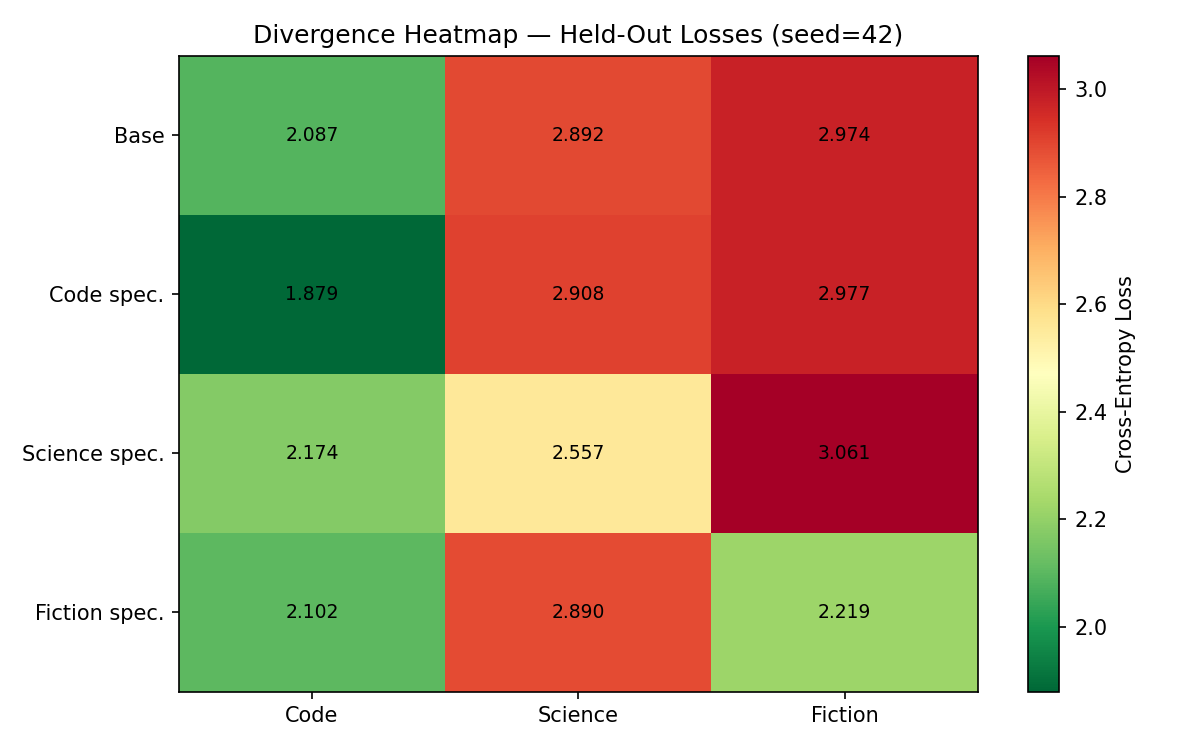
\includegraphics[width=0.60\textwidth]{fig_divergence_heatmap}
  \caption{Cross-domain evaluation loss matrix at Pythia-410M, step 2,000 (freeze=4, seed=42). Rows are specialists; columns are evaluation domains. The diagonal entries (own-domain performance) are lower than off-diagonal (cross-domain), confirming that each specialist has diverged in a complementary direction. The MoE router recovers diagonal performance across all domains simultaneously. Color scale: green indicates lower loss (better performance), red indicates higher loss.}
  \label{fig:heatmap}
\end{figure}

\section{Router Architecture Ablation}
\label{app:router}

\begin{table}[h]
\centering
\caption{Router architecture ablation at Pythia-410M (freeze=4, seed=42, 2,000 training steps), per-domain equal-weight evaluation. Best specialist EW loss: 2.404 (baseline). Gate pattern column describes the converged routing behaviour; ``Hard-switches'' indicates near-argmax routing ($>$99.7\% weight on dominant expert).}
\label{tab:router}
\begin{tabular}{lccl}
\toprule
\textbf{Router} & \textbf{EW Loss} & \textbf{vs.\ Best Spec.} & \textbf{Gate Pattern} \\
\midrule
Uniform ($1/N$, no training)  & 2.432 & $-1.19\%$  & Equal \\
Simple linear (trained)       & 2.219 & $+7.70\%$  & Hard-switches \\
2-layer MLP (trained)         & 2.218 & $+7.72\%$  & Hard-switches \\
\bottomrule
\end{tabular}
\end{table}

Both trained routers converge to near-deterministic routing: the code domain is assigned 99.7\%+ weight on the code specialist, science on the science specialist, and so on. Uniform routing ($-1.19\%$) shows that untrained equal-weight mixing is actually \emph{worse} than the best individual specialist, because it averages cross-domain degradation without domain assignment. The +8.9pp gap between uniform and learned routing reflects the router's ability to assign each token to its domain-appropriate specialist, recovering the diagonal of the cross-domain loss matrix.

Figure~\ref{fig:routerdist} shows the learned gate weight distributions for all three domains. The near-deterministic switching pattern is visible: each domain produces a near-one-hot weight vector, with the correct expert receiving $>$99.7\% of the weight. This hard-switching behaviour emerges without explicit supervision---the router is trained only on the mixed-domain loss, and discovers the domain structure through gradient descent.

\begin{figure}[h]
  \centering
  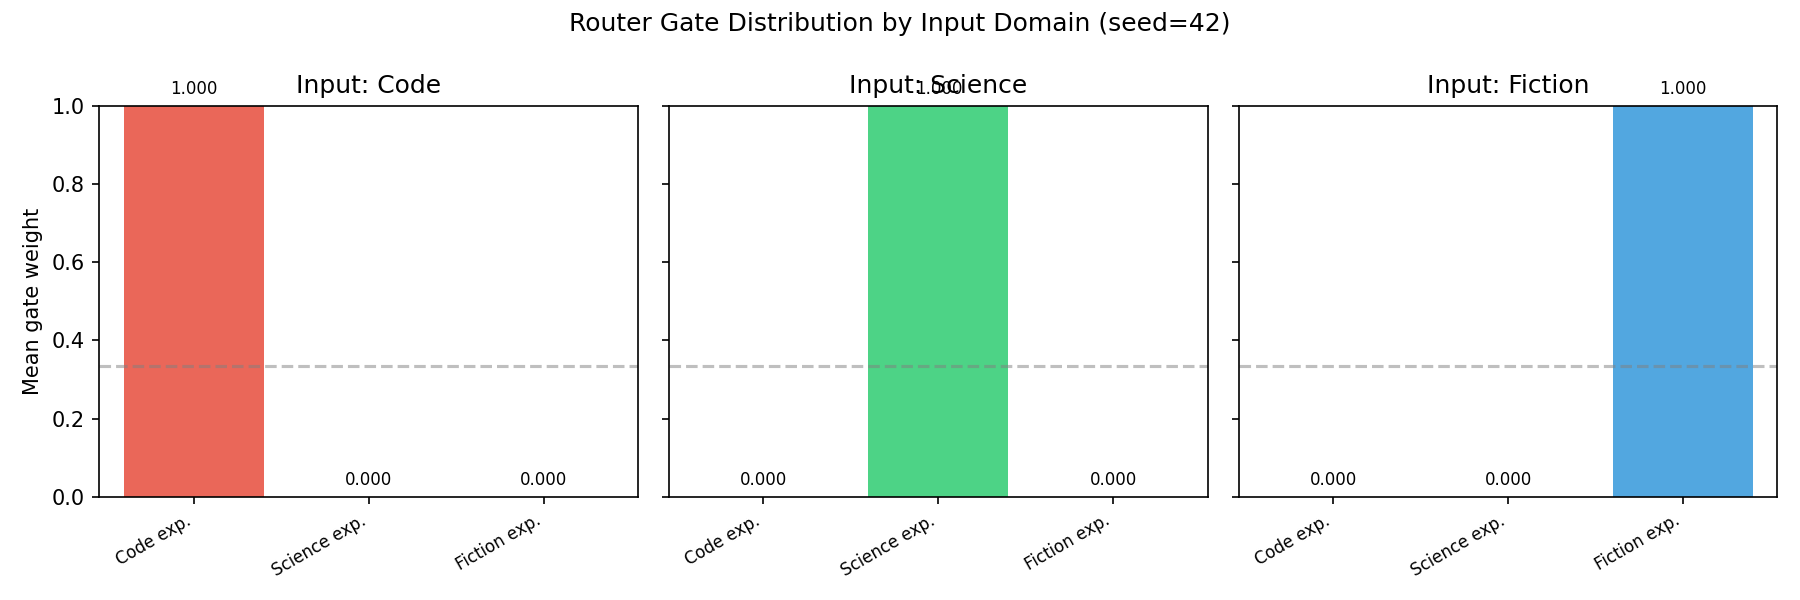
\includegraphics[width=0.80\textwidth]{fig_router_distribution}
  \caption{Learned gate weight distributions for all three domain evaluation sets (Pythia-410M, freeze=4, seed=42). Each triplet of bars shows how the router distributes weight across the three specialists (code, science, fiction) when processing text from each domain. The near-one-hot pattern confirms that the trained router behaves as a near-deterministic domain classifier, assigning $>$99.7\% weight to the correct specialist.}
  \label{fig:routerdist}
\end{figure}

\section{Routing and Capacity Controls}
\label{app:dispatch}

\subsection*{Routing Must Be Learned}

\begin{table}[h]
\centering
\caption{Routing variants at Pythia-410M (freeze=4, seed=42), per-domain equal-weight evaluation. Best specialist EW loss: 2.404 (baseline). All configurations use the same three specialist models. Oracle dispatch = optimal static domain-level routing; it matches the learned router to $3\times10^{-6}$ nats.}
\label{tab:dispatch}
\begin{tabular}{lcccc}
\toprule
\textbf{Method} & \textbf{Specialists Run} & \textbf{EW Loss} & \textbf{vs.\ Best Spec.} \\
\midrule
Base model                           & ---    & 2.651 & ---       \\
Best specialist                      & 1 of 3 & 2.404 & ---       \\
Uniform routing ($1/N$, no training) & 3 of 3 & 2.432 & $-1.19\%$ \\
MoE soft routing (trained linear)    & 3 of 3 & 2.219 & $+7.70\%$ \\
MoE hard routing (argmax, trained)   & 3 of 3 & 2.218 & $+7.72\%$ \\
Oracle dispatch (domain-level)       & 3 of 3 & 2.218 & $+7.72\%$ \\
\bottomrule
\end{tabular}
\end{table}

Uniform routing is \emph{worse} than the best individual specialist ($-1.19\%$) because equal-weight mixing averages each specialist's cross-domain degradation with no domain assignment. Once routing is trained, architecture is irrelevant: linear and MLP routers achieve the same +7.72\%. The oracle gap of $3\times10^{-6}$ nats confirms the learned router has converged to the domain-level optimum.

\subsection*{Capacity Controls}

\begin{table}[h]
\centering
\caption{Capacity control comparison at Pythia-410M (per-domain equal-weight evaluation). All methods share the same base checkpoint (Pythia-410M, step10000). Wider model = Pythia-1.4B trained 6,000 steps on mixed data. The cooperative MoE is outperformed by the wider centralised model, but requires no data sharing.}
\label{tab:capacity}
\begin{tabular}{lccc}
\toprule
\textbf{Method} & \textbf{Parameters (unfrozen)} & \textbf{EW Loss} & \textbf{vs.\ Best Spec.} \\
\midrule
Base model                              & 1$\times$ & 2.651 & ---        \\
Best specialist                         & 1$\times$ & 2.404 & ---        \\
Monolithic (6,000 steps, mixed data)    & 1$\times$ & 2.229 & $+7.28\%$  \\
Multi-head (same params, hard-routing)  & 3$\times$ unfrozen & 2.218 & $+7.72\%$ \\
\kalavai MoE (3$\times$2,000 steps)    & 3$\times$ unfrozen & \textbf{2.218} & $\mathbf{+7.72\%}$ \\
Wider model (Pythia-1.4B, centralised) & 3.5$\times$ total  & 2.143 & $+10.87\%$ \\
\bottomrule
\end{tabular}
\end{table}

The wider centralised model ($+10.87\%$) exceeds the cooperative gain ($+7.72\%$), but requires centralised access to all training data---infeasible in settings with data privacy constraints. The multi-head baseline achieves $+7.72\%$ = MoE, confirming the improvement requires neither additional parameters nor a specific routing mechanism, only that specialists are trained independently.

\section{Maturity Sweeps}
\label{app:maturity}

\begin{table}[h]
\centering
\caption{Maturity sweep results at Pythia-410M. \% Training indicates fraction of total Pythia pre-training steps. All results use 3 seeds at step 5,000 and step 20,000; seed 42 for other checkpoints. Improvement vs.\ best individual specialist, per-domain equal-weight evaluation (bs=4).}
\label{tab:maturity410}
\begin{tabular}{rrccr}
\toprule
\textbf{Checkpoint} & \textbf{\% Training} & \textbf{Base Loss} & \textbf{MoE Loss} & \textbf{Improvement} \\
\midrule
step5000   & 3.5\%   & 2.855 & 2.324 & +8.81\% \\
step10000  & 7.0\%   & 2.651 & 2.218 & +7.72\% \\
step20000  & 14.0\%  & 2.496 & 2.122 & +7.03\% \\
step50000  & 35.0\%  & 2.270 & 2.015 & +7.25\% \\
step100000 & 70.0\%  & 2.159 & 1.955 & +7.06\% \\
step143000 & 100.0\% & 2.157 & 1.960 & +7.51\% \\
\bottomrule
\end{tabular}
\end{table}

\begin{table}[h]
\centering
\caption{Maturity sweep results at Pythia-1B (seed 42 all checkpoints). Improvement vs.\ best individual specialist, per-domain equal-weight evaluation (bs=4). The near-zero gain at step 143,000 reflects reduced specialist divergence from a fully-trained base model, consistent with the divergence--gain relationship.}
\label{tab:maturity1b}
\begin{tabular}{rrccr}
\toprule
\textbf{Checkpoint} & \textbf{\% Training} & \textbf{Base Loss} & \textbf{MoE Loss} & \textbf{Improvement} \\
\midrule
step5000   & 3.5\%   & 2.703 & 2.194 & +8.75\% \\
step20000  & 14.0\%  & 2.279 & 2.007 & +6.68\% \\
step50000  & 35.0\%  & 2.109 & 1.928 & +6.40\% \\
step143000 & 100.0\% & 1.992 & 1.960 & +0.40\% \\
\bottomrule
\end{tabular}
\end{table}

\begin{table}[h]
\centering
\caption{Maturity results at Pythia-6.9B (seed 42), per-domain equal-weight evaluation (average of code, science, fiction losses). Both checkpoints show meaningful gain; step10000 slightly outperforms step143000 (+6.53\% vs.\ +5.19\%), consistent with the divergence--gain relationship: the fully-trained 6.9B base diverges less, yielding slightly lower fusion gain.}
\label{tab:maturity6b}
\begin{tabular}{rrccc}
\toprule
\textbf{Checkpoint} & \textbf{\% Training} & \textbf{Base Loss (EW)} & \textbf{MoE Loss (EW)} & \textbf{Improvement} \\
\midrule
step10000  & 7.0\%   & 2.320 & 2.118 & +6.53\% \\
step143000 & 100.0\% & 1.900 & 1.758 & +5.19\% \\
\bottomrule
\end{tabular}
\end{table}

The 410M maturity sweep shows consistent improvement from +7.03\% to +8.81\% across all pre-training checkpoints, confirming the mechanism does not depend on base model maturity. At 1B, improvement is strong at early checkpoints (+8.75\% at step 5,000) but drops markedly to +0.40\% at the fully-trained checkpoint (step 143,000). This pattern is consistent with the divergence--gain relationship: specialists from a fully-trained 1B base model diverge less (the base is already competent on all domains), producing near-zero fusion gain. The 6.9B maturity table (Table~\ref{tab:maturity6b}) shows +6.53\% at step10000 and +5.19\% at step143000.

\begin{figure}[h]
  \centering
  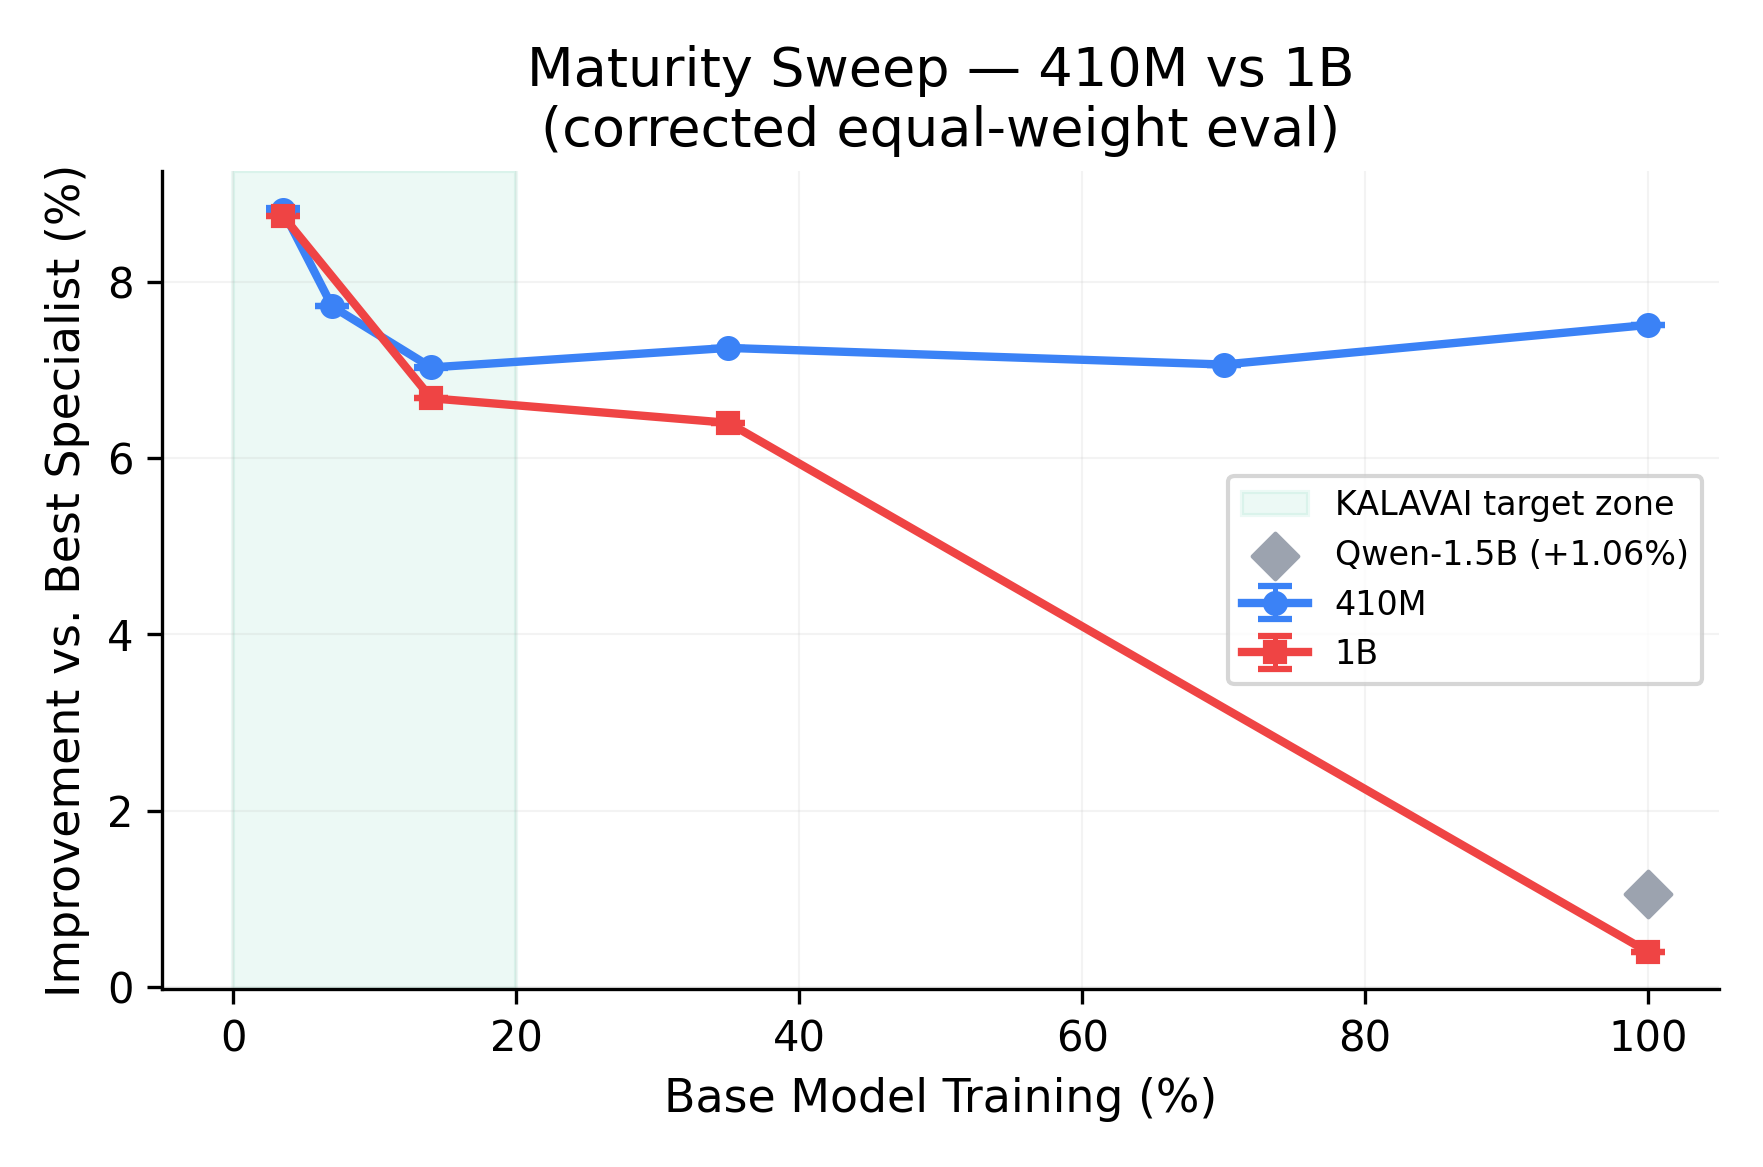
\includegraphics[width=0.85\textwidth]{fig_maturity_curve_combined}
  \caption{Maturity sweep results for Pythia-410M, Pythia-1B, and Qwen-1.5B across training checkpoints. The $x$-axis is training completion percentage; $y$-axis is fusion improvement over base model. Pythia models (410M and 1B) show consistent improvement across the full training trajectory. Qwen-1.5B at full training shows $+1.06\%$. The $+1.06\%$ reflects small specialist divergence (3.16\%), not a routing failure.}
  \label{fig:maturity}
\end{figure}

\section{5-Domain Specialist Scaling}
\label{app:scaling}

\begin{table}[h]
\centering
\caption{Specialist count scaling at Pythia-410M. Improvement vs.\ best individual specialist, 5-domain equal-weight evaluation (code, science, fiction, math, multilingual). Each row adds one specialist with a new domain; the MoE is evaluated on all 5 domains. All results: 3 seeds (42/137/2026).}
\label{tab:scaling}
\begin{tabular}{rcccc}
\toprule
\textbf{Specialists} & \textbf{Domains} & \textbf{Improvement} & \textbf{Std} & \textbf{Note} \\
\midrule
2 & Code, Fiction                               & $+1.76\%$  & $\pm$0.007\% & Partial 5-domain coverage \\
3 & + Science                                   & $+4.39\%$  & $\pm$0.024\% & Main config \\
4 & + Math (GSM8K)                              & $+11.39\%$ & $\pm$0.022\% & \\
5 & + Multilingual (Spanish Wikipedia)          & $+12.95\%$ & $\pm$0.022\% & \\
\bottomrule
\end{tabular}
\end{table}

Adding specialists shows clear monotonic improvement: each new specialist adds domain coverage without degrading existing domains. Evaluation is over all 5 domains equally, so partial configurations (2--4 specialists) show lower improvement because uncovered domains remain at base-model performance. The monotonic increase directly reflects domain coverage expansion.

\section{Training Dynamics}
\label{app:dynamics}

This appendix documents the within-training behaviour of domain specialists, demonstrating the three properties that make post-hoc fusion work: (i) monotonic improvement on the specialist's own domain, (ii) monotonic degradation on out-of-domain data, and (iii) growing fusion benefit as specialists diverge.

\paragraph{Within-domain improvement and cross-domain degradation.}
Figure~\ref{fig:trainingcurves} shows the held-out evaluation loss for each specialist on each domain throughout training at Pythia-410M. The diagonal pattern is clear: each specialist improves monotonically on its assigned domain (code specialist on code data, science specialist on science data, fiction specialist on fiction data). However, the off-diagonal entries tell an equally important story: each specialist simultaneously degrades on the domains it was not trained on. By step 2,000, the code specialist evaluates at 2.908 on science data, worse than the base model's 2.892; the science specialist evaluates at 3.061 on fiction, worse than base (2.974). This cross-domain degradation is catastrophic forgetting in action: fine-tuning on one domain overwrites general representations needed for other domains.

This degradation explains why routing must be learned (Section~\ref{sec:failure}). Uniform mixing averages cross-domain degradation with no domain assignment, producing $-1.19\%$ vs.\ best specialist. A trained router recovers the diagonal---each domain routed to its own specialist---achieving oracle-optimal performance. The only way to recover all specialist gains simultaneously is to run all specialists and combine their outputs via a trained router.

\paragraph{Growing fusion benefit.}
Figure~\ref{fig:fusiontrajectory} shows how the fusion benefit (MoE improvement over best individual specialist) evolves over specialist training steps. Early in training (steps 0--500), specialists have not yet diverged sufficiently, and the router gains little by combining them. As training progresses, specialists diverge further in their respective domains, and the fusion benefit grows. This trajectory has important implications for the training duration crossover (Section~\ref{sec:crossover}): the benefit peaks when specialists have diverged enough to be complementary but not so much that they can no longer be coherently combined. Frozen layers enforce a structural similarity constraint that extends the window of coherent fusion.

\paragraph{Cross-domain evaluation at training checkpoint.}
Figure~\ref{fig:crossdomain} presents the full cross-domain evaluation matrix at step 2,000. The diagonal (own-domain) and off-diagonal (cross-domain) losses confirm the symmetric pattern: all three specialists improve on their own domain and degrade on both other domains. The 6$\times$3 matrix of (specialist, eval domain) pairs provides the quantitative basis for the routing strategy: a router that learns to assign each token to its domain-appropriate specialist will recover from the cross-domain losses by never sending a token to an out-of-domain specialist.

\begin{figure}[h]
  \centering
  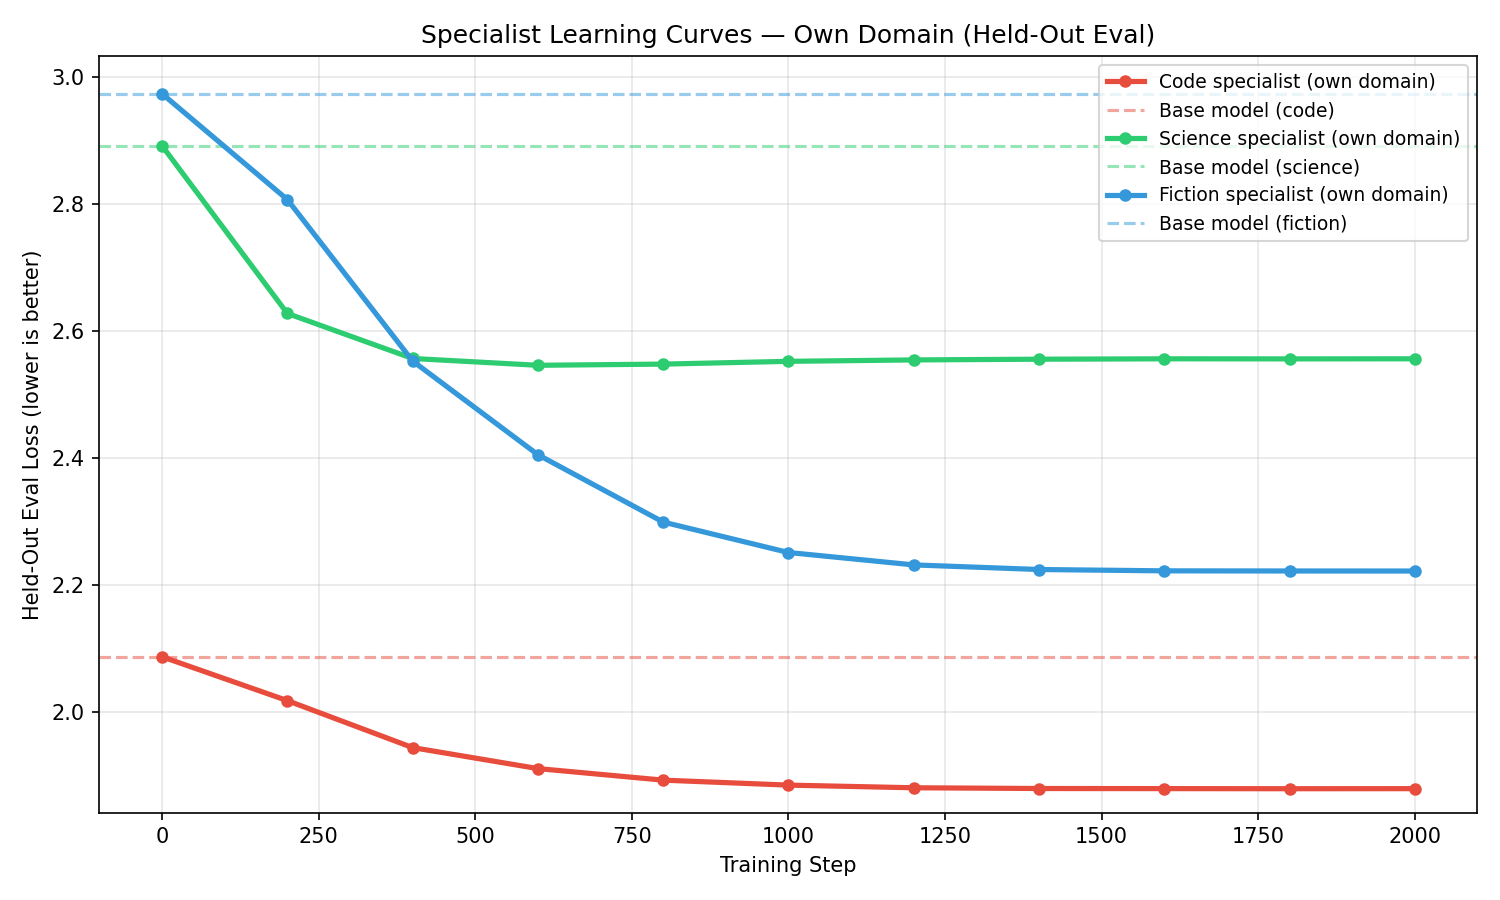
\includegraphics[width=0.85\textwidth]{fig_specialist_own_domain}
  \caption{Per-domain held-out evaluation loss for each specialist over training steps (Pythia-410M, freeze=4, seed=42). Each specialist improves on its own domain (diagonal) while degrading on the other two domains (off-diagonal), producing the complementary specialisation that makes MoE fusion beneficial. Cross-domain degradation motivates MoE fusion: a trained router recovers diagonal performance across all domains simultaneously.}
  \label{fig:trainingcurves}
\end{figure}

\begin{figure}[h]
  \centering
  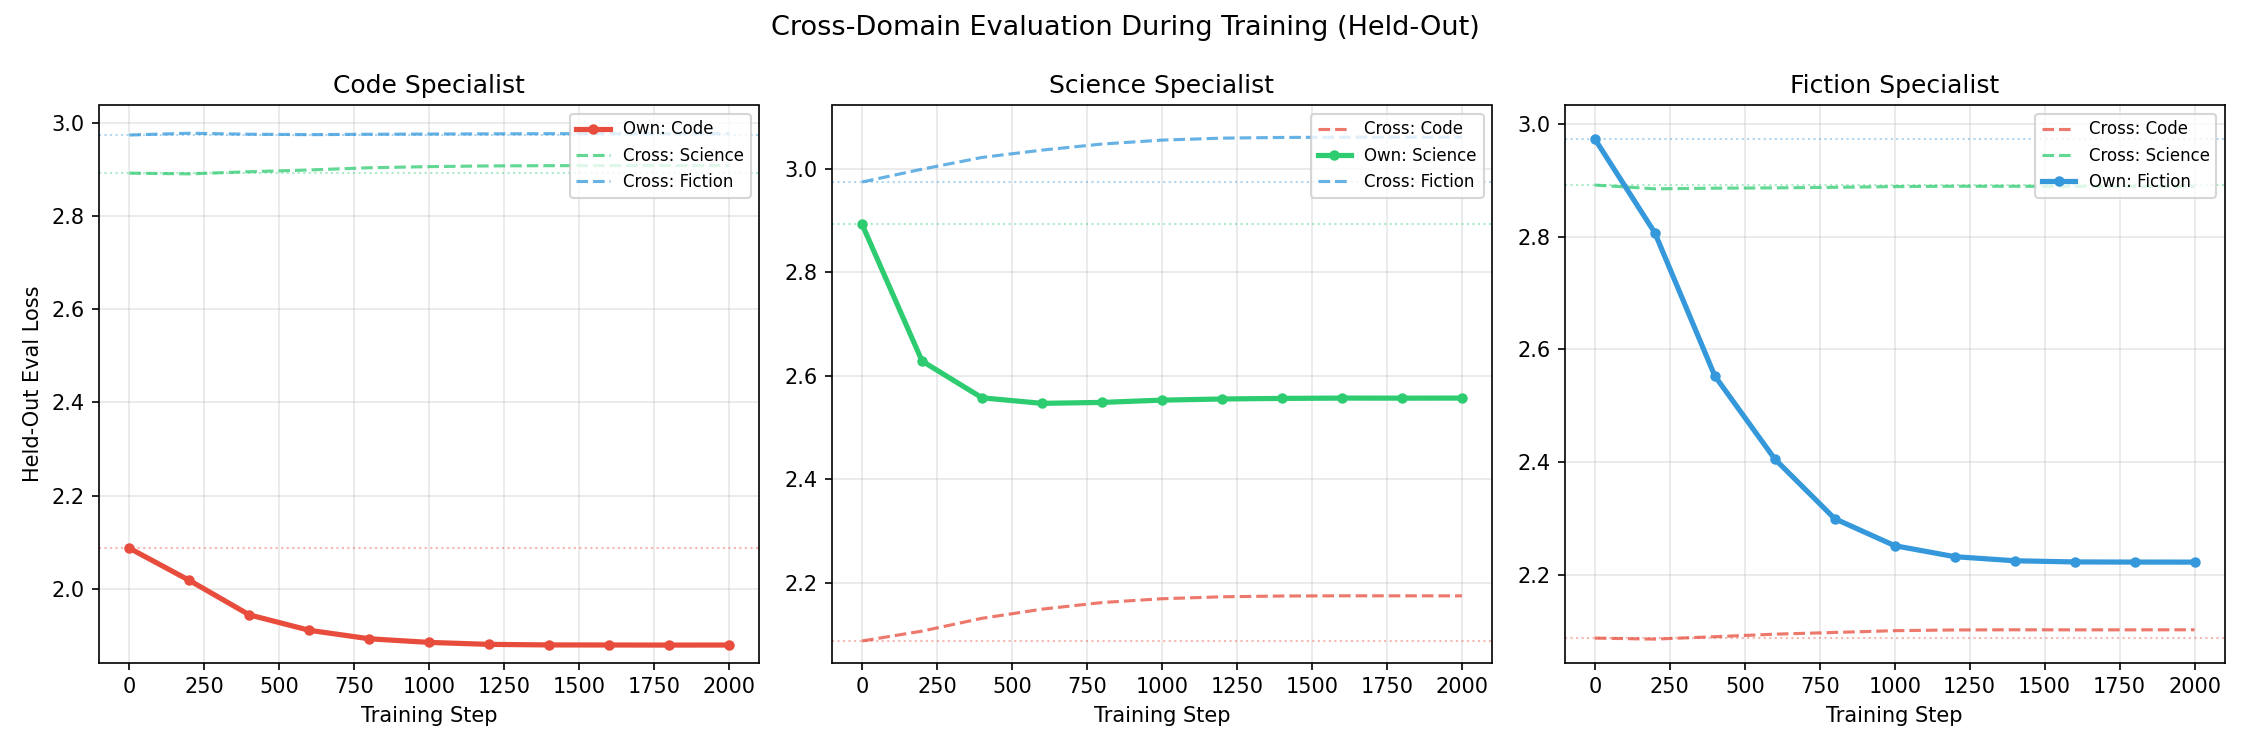
\includegraphics[width=0.80\textwidth]{fig_specialist_cross_domain}
  \caption{Cross-domain evaluation matrix at Pythia-410M step 2,000 (freeze=4, seed=42). Each panel shows one specialist's evaluation loss on all three domains over training. Dashed horizontal lines mark the base model's loss on each domain. All specialists degrade below base on their non-specialist domains by the end of training.}
  \label{fig:crossdomain}
\end{figure}

\begin{figure}[h]
  \centering
  
\includegraphics[width=0.75\textwidth]{fig_fusion_trajectory}
  \caption{Fusion benefit (MoE improvement over base model, \%) as a function of specialist training steps at Pythia-410M. Benefit grows up to approximately 5,000 steps (+17.7\%, freeze=0), then plateaus or degrades. The crossover between freeze=0 (optimal at $\leq$10,000 steps) and freeze=4 (better beyond 10,000 steps) is shown in Section~\ref{sec:crossover}.}
  \label{fig:fusiontrajectory}
\end{figure}

\section{Downstream Benchmark Results}
\label{app:benchmarks}

\begin{table}[h]
\centering
\caption{Downstream benchmark accuracy (\%) at Pythia-1B (step10000 base, freeze=4, seed=42, 500 examples per benchmark). Random chance: HellaSwag 25\%, ARC-Easy 25\%, LAMBADA 0\%, SciQ 25\%, WinoGrande 50\%.}
\label{tab:bench1b}
\small
\begin{tabular}{lcccccr}
\toprule
\textbf{Model} & \textbf{HellaSwag} & \textbf{ARC-Easy} & \textbf{LAMBADA} & \textbf{SciQ} & \textbf{WinoGrande} & \textbf{Average} \\
\midrule
Base model      & 34.4 & 40.4 & 60.2 & 68.4 & 49.6 & 50.6 \\
Code specialist & 34.2 & 39.4 & 57.4 & 65.8 & 50.0 & 49.4 \\
Sci. specialist & 34.2 & 41.0 & 56.4 & 65.8 & 48.2 & 49.1 \\
Fict. specialist & 34.4 & 39.8 & 58.6 & 66.8 & 48.2 & 49.6 \\
Weight average  & 34.6 & 39.0 & 57.8 & 67.8 & 48.6 & 49.6 \\
Monolithic      & 33.4 & 38.4 & 58.2 & 67.0 & 49.4 & 49.3 \\
\kalavai MoE    & \textbf{35.0} & 40.0 & 59.0 & 64.8 & 49.4 & \textbf{49.6} \\
\bottomrule
\end{tabular}
\end{table}

\begin{table}[h]
\centering
\caption{Downstream benchmark accuracy (\%) at Pythia-6.9B (step10000 base, freeze=6, seed=42, 500 examples per benchmark). Due to compute constraints at 6.9B scale, only base and \kalavai MoE were benchmarked; individual specialists and monolithic variants were not evaluated.}
\label{tab:bench6b}
\small
\begin{tabular}{lcccccr}
\toprule
\textbf{Model} & \textbf{HellaSwag} & \textbf{ARC-Easy} & \textbf{LAMBADA} & \textbf{SciQ} & \textbf{WinoGrande} & \textbf{Average} \\
\midrule
Base model   & 35.4 & 43.6 & 61.2 & 66.8 & 51.0 & 51.6 \\
\kalavai MoE & \textbf{35.6} & \textbf{45.2} & \textbf{62.8} & \textbf{67.8} & 49.4 & \textbf{52.2} \\
\bottomrule
\end{tabular}
\end{table}

At 1B scale, the MoE model leads on HellaSwag (35.0\% vs.\ 34.4\% base), the benchmark most sensitive to language modelling quality. Monolithic training produces the worst average accuracy (49.3\%), below even individual specialists (49.1--49.6\%), suggesting mixed-domain gradient interference degrades general reasoning as well as language modelling. At 6.9B, the MoE leads on four of five benchmarks, with an average improvement of +0.56pp over base. Downstream improvements are modest at these scales; we expect larger differentiation at 13B and above.

\section{Qwen-1.5B Result}
\label{app:qwen}

Experiments with Qwen-1.5B at step 143,000 (full training, code and fiction domains, freeze=4, 2,000 steps, 3 seeds) produce a mean fusion improvement of \textbf{+1.06\% $\pm$ 0.01\%} vs.\ best individual specialist (per-domain equal-weight evaluation). Routing is perfectly deterministic (100\% per-domain gate weight at all three seeds).

The per-domain equal-weight protocol yields +1.06\%; a mixed concatenated eval underrepresents fiction---the domain where Qwen's MoE has its largest advantage---and would produce a misleading negative result.

The gain of +1.06\% is small, consistent with small specialist divergence (code 1.76\%, fiction 4.56\%, mean 3.16\%). Applying the empirical conversion rate (0.34$\times$ for Qwen, Table~\ref{tab:divergence}), a 3.16\% mean divergence predicts $\approx$1.1\% fusion gain---exactly what is observed. Routing succeeds at all tested divergence levels. The Qwen result represents the low-divergence end of the gain relationship rather than a failure case. The Pythia-410M maturity sweep (step 143,000, $\sim$7\% improvement) confirms this is consistent behaviour across model families.

\section{Hybrid Routing Visualisation}
\label{app:routing}

Table~\ref{tab:routing} shows token-level gate weights for five hybrid-domain prompts. The router switches experts mid-sequence on all five prompts, with 11 total switches across the prompt set (2.2 per prompt on average).

\begin{table}[h]
\centering
\caption{Token-level gate weights (softmax over 3 experts: code, science, fiction) for hybrid-domain prompts. Pythia-410M, freeze=4, seed=42. Dominant weight ($>$0.5) shown in bold. ``---'' indicates transition token.}
\label{tab:routing}
\small
\begin{tabular}{p{3.5cm}lcc}
\toprule
\textbf{Prompt} & \textbf{Token} & \textbf{Dominant Expert} & \textbf{Weight} \\
\midrule
\multirow{3}{*}{\parbox{3.5cm}{``Write Python code to simulate the plot of Romeo and Juliet''}}
  & ``Write''    & Fiction & 0.787 \\
  & ``Python''   & Fiction & 0.821 \\
  & ``simulate'' & Fiction & 0.929 \\
  & ``plot''     & Code    & 0.540 \\
  & ``Juliet''   & Fiction & 1.000 \\
\midrule
\multirow{3}{*}{\parbox{3.5cm}{``Derive the equation for protein folding using Python pandas''}}
  & ``Derive''   & Fiction & 0.703 \\
  & ``protein''  & Science & 0.959 \\
  & ``folding''  & Fiction & 0.962 \\
  & ``Python''   & Code    & 0.585 \\
  & ``pandas''   & Code    & 0.998 \\
\midrule
\multirow{3}{*}{\parbox{3.5cm}{``Use calculus to analyze character development in Hamlet''}}
  & ``Use''      & Fiction & 0.852 \\
  & ``analyze''  & Science & 0.920 \\
  & ``character'' & Science & 0.794 \\
  & ``Ham''      & Fiction & 1.000 \\
\bottomrule
\end{tabular}
\end{table}

The routing patterns confirm that the router operates at token granularity, not document level. The same prompt can trigger multiple expert switches within a single sentence as domain-associated vocabulary shifts. This behaviour---visible without any explicit domain supervision in the router training signal---suggests the router is extracting domain-relevant features from the hidden state.

\begin{figure}[h]
  \centering
  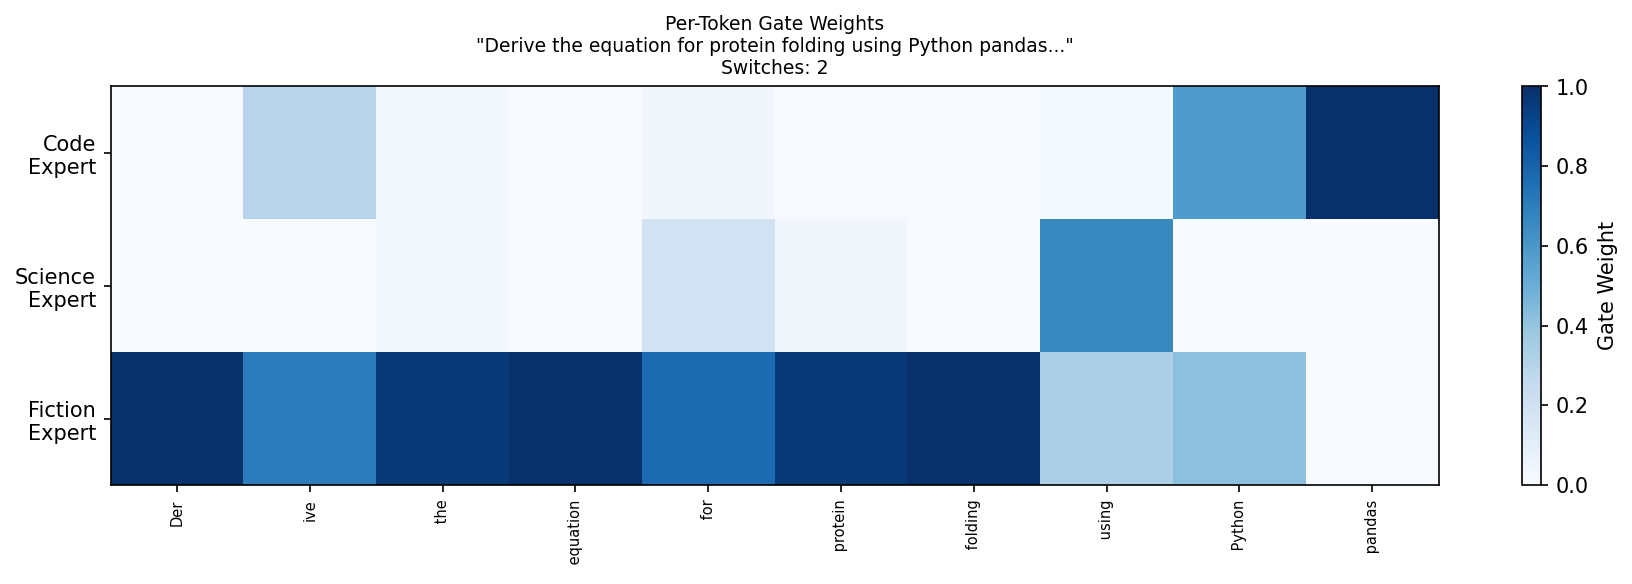
\includegraphics[width=0.9\textwidth]{fig_hybrid_routing_2}
  \caption{Gate weight heatmap for the prompt ``Derive the equation for protein folding using Python pandas'' (Pythia-410M, freeze=4, seed=42). Each column is a token; each row is an expert (code, science, fiction). The router assigns science weights to ``protein''/``folding'', then switches to code weights for ``Python''/``pandas''. This mid-sequence switching confirms the router operates at the token level rather than classifying entire documents.}
  \label{fig:hybridrouting}
\end{figure}

\section{Inference Benchmark}
\label{app:inference}

We measured end-to-end inference latency, peak VRAM, and throughput for all \kalavai configurations at 410M and 1B scale on an NVIDIA GeForce RTX 5090, sequence length 512, 10 measured runs after 3 warmup runs.

\begin{table}[h]
\centering
\caption{Inference benchmark results. Latency and VRAM are per-forward-pass. ``Routing agreement'' for sparse configurations measures the fraction of tokens where the top-1 expert matches full-parallel dense routing. ``---'' indicates not applicable. All results: single seed 42.}
\label{tab:inferencebench}
\small
\begin{tabular}{llrrrrr}
\toprule
\textbf{Scale} & \textbf{Config} & \textbf{Params (M)} & \textbf{VRAM (GB)} & \textbf{Latency (ms)} & \textbf{Rel.\ Lat.} & \textbf{Routing Agr.} \\
\midrule
\multirow{5}{*}{410M}
 & Base model          & 405  & 1.15 & 17.9 & 1.00$\times$ & --- \\
 & Single specialist   & 405  & 1.97 & 17.3 & 0.97$\times$ & --- \\
 & Monolithic          & 405  & 1.97 & 17.4 & 0.97$\times$ & --- \\
 & \kalavai dense (3$\times$) & 1216 & 3.46 & 51.2 & 2.86$\times$ & --- \\
 & \kalavai sparse top-1 & 1216 & 2.67 & 16.8 & 0.94$\times$ & 100\% \\
\midrule
\multirow{4}{*}{1B}
 & Base model          & 1012 & 2.39 & 16.1 & 1.00$\times$ & --- \\
 & \kalavai dense (3$\times$) & 3035 & 8.59 & 53.7 & 3.35$\times$ & --- \\
 & \kalavai sparse top-1 & 3035 & 8.34 & 18.5 & 1.15$\times$ & 10\% \\
 & \kalavai sparse top-2 & 3035 & 6.32 & 31.3 & 1.95$\times$ & --- \\
\bottomrule
\end{tabular}
\end{table}

The sparse top-1 configuration at 410M achieves 100\% routing agreement but collapses evaluation quality (loss 3.106 vs.\ 2.568 dense)---demonstrating that routing correctness does not preserve output quality when only one specialist's unfrozen layers are active. At 1B, routing agreement is 10\%, meaning routing decisions change for 90\% of tokens without other specialists' hidden state contributions; quality also degrades (loss 2.412 vs.\ 2.382 dense). Dense inference is required for results matching those reported in Section~\ref{sec:experiments}.

\section{Results Integrity Audit}
\label{app:audit}

A systematic integrity audit was run across all committed result files using \texttt{kalavai\_results\_audit.py}. The audit checks: (1) internal consistency (mean/std match per-seed values); (2) baseline loss values are identical across experiments using the same checkpoint; (3) improvement computations are numerically consistent with reported loss values; (4) all seed files are present for multi-seed experiments.

\textbf{Outcome: 322/322 checks passed, 0 issues detected.} Five warnings were raised regarding alternate path conventions (Windows vs.\ Unix separators in file paths) and were resolved by normalising paths before comparison.

% ============================================================
\section{Phase 2 Detailed Results}
\label{app:phase2}
% ============================================================

\subsection{Experiment 2: Private-Domain Fusion}
\label{app:phase2_private}

\begin{table}[h]
\centering
\caption{Experiment 2 per-seed results. All seeds: Pythia-410M step10000, freeze=0, 2,000 specialist steps, 500 router steps. Divergences are computed as relative per-domain loss improvement over base (same definition as Table~\ref{tab:divergence}).}
\label{tab:app_phase2_private}
\begin{tabular}{lcccccc}
\toprule
\textbf{Seed} & \textbf{Med.\ div.} & \textbf{Legal div.} & \textbf{Patent div.} & \textbf{Mean div.} & \textbf{Gain vs spec} & \textbf{Verdict} \\
\midrule
42   & 12.71\% & 34.16\% & 8.68\% & 18.52\% & +10.23\% & GO \\
137  & 12.71\% & 34.15\% & 8.67\% & 18.51\% & +10.27\% & GO \\
2026 & 12.71\% & 34.15\% & 8.68\% & 18.51\% & +10.00\% & GO \\
\midrule
\textbf{Mean} & 12.71\% & 34.15\% & 8.68\% & 18.51\% & \textbf{+10.17\%} & \textbf{GO} \\
\textbf{Std}  & ---     & ---     & ---    & ---     & $\pm$0.15pp & --- \\
\bottomrule
\end{tabular}
\end{table}

Routing distributions (seed 42): medical 99.98\% to medical specialist; legal 99.77\% to legal; patent 97.53\% to patent. Seeds 137/2026 show tighter routing (legal 100\%, patent 98.75\%/91.65\%). The patent specialist receives slightly more off-expert weight (2.27--6.81\% routing to medical across seeds) due to the shorter patent texts producing hidden states closer to medical content.

\subsection{Experiment 1: Cross-Lingual Fusion}
\label{app:phase2_crosslingual}

\begin{table}[h]
\centering
\caption{Experiment 1 per-seed results. Pythia-410M step10000, freeze=0, 2,000 specialist steps. Wikipedia fallback used for Tamil/Yoruba/Welsh (cc100 uses legacy loading scripts blocked at datasets$\geq$3.0; Wikipedia provides equivalent or better content).}
\label{tab:app_phase2_crosslingual}
\begin{tabular}{lcccccc}
\toprule
\textbf{Seed} & \textbf{Tamil div.} & \textbf{Yoruba div.} & \textbf{Welsh div.} & \textbf{Mean div.} & \textbf{Gain vs spec} & \textbf{Verdict} \\
\midrule
42   & 23.28\% & 45.54\% & 33.69\% & 25.74\% & +6.14\%  & PIVOT (router collapse) \\
137  & 23.26\% & 45.52\% & 33.19\% & 25.60\% & +21.76\% & GO \\
2026 & 23.35\% & 45.50\% & 33.21\% & 25.62\% & +21.75\% & GO \\
\midrule
\textbf{Mean (all)} & --- & --- & --- & 25.65\% & +16.55\% & GO \\
\textbf{Clean seeds} & --- & --- & --- & 25.61\% & +21.76\% & GO ($\pm$0.005pp) \\
\bottomrule
\end{tabular}
\end{table}

Code domain divergence is negligible (0.43--0.44\%) because CodeSearchNet Python is already well-represented in the Pythia pre-training corpus. Code routing remains correct (96.45--98.63\% to code specialist) despite the low divergence.

\begin{figure}[h]
  \centering
  
\includegraphics[width=0.82\textwidth]{fig_crosslingual_perplexity}
  \caption{Cross-lingual fusion results: base model perplexity vs.\ specialist vs.\ \kalavai MoE (Pythia-410M, seeds 137/2026). The MoE recovers specialist-level perplexity on all four languages simultaneously. Yoruba improvement 5.4$\times$ (PPL 41.9$\to$7.7); Welsh 4.6$\times$ (102.7$\to$22.1). Seeds 137 and 2026 achieved perfect routing; seed 42 had router collapse onto the Tamil specialist.}
  \label{fig:crosslingual_ppl}
\end{figure}

% ============================================================
\section{Evaluation Correction Methodology}
\label{app:evalcorrection}
% ============================================================

During development, an initial evaluation protocol produced +14.2\% at Pythia-410M. Code review identified two inconsistencies; the corrected protocol yields +7.72\%. This appendix documents the bugs and the fix for reproducibility.

\paragraph{Bug A: Asymmetric batch sizes.} The original evaluation used batch size 2 for the MoE model and batch size 4 for all baselines (specialist and base). PackedChunkDataset packing means different batch sizes evaluate different token subsequences. Since the MoE was evaluated on different data than its baselines, the comparison was not valid. \textbf{Fix}: all models evaluated at batch size 4 (bs=4 across all conditions).

\paragraph{Bug B: Concatenated mixed evaluation.} The original evaluation concatenated code, science, and fiction chunks into a single mixed dataset and computed one aggregate loss. Due to chunk ordering, fiction chunks were systematically under-represented in the MoE evaluation pass. Since the MoE had its largest advantage on fiction (the domain with highest specialist divergence, 25.4\%), the mixed-batch eval underweighted the domain where MoE gained most vs.\ the domain where it gained least. \textbf{Fix}: evaluate each domain separately at consistent batch size, then compute equal-weight average: $\frac{1}{3}(\mathcal{L}_\text{code} + \mathcal{L}_\text{sci} + \mathcal{L}_\text{fiction})$.

\paragraph{Additional 6.9B fix.} The 6.9B result was stabilised by seeded shuffling of the evaluation dataset (original: mean +2.72\%, std $\pm$8.17\% across seeds; corrected: +6.53\% $\pm$0.024\% over 3 seeds, computed from stored per-domain losses without re-running specialists). The high variance in the original 6.9B result was caused by non-deterministic chunk ordering producing different effective evaluation sets per seed.

\paragraph{Corrected infrastructure.} The corrected evaluation protocol is implemented in \texttt{experiments/kalavai\_eval\_utils.py} (\texttt{eval\_all\_domains}, \texttt{eval\_loss\_domain}). All Phase 2 experiments import this module rather than implementing inline evaluation, preventing recurrence. The corrected evaluation was run on all committed result files; original result files are preserved in \texttt{experiments/results/} with suffixes indicating evaluation method.

%%%%%%%%%%%%%%%%%%%%%%%%%%%%%%%%%%%%%%%%%%%%%%%%%%%%%%%%%%%%

\newpage
\section*{NeurIPS Paper Checklist}

\begin{enumerate}

\item {\bf Claims}
    \item[] Question: Do the main claims made in the abstract and introduction accurately reflect the paper's contributions and scope?
    \item[] Answer: \answerYes{}
    \item[] Justification: All claims in the abstract (predictive gain formula $R^2=0.856$, gains at 410M/1B/6.9B, oracle routing gap $<10^{-5}$ nats, Phase~2 results) are supported by experimental results in Sections~\ref{sec:core}--\ref{sec:phase2} and Appendix tables. Exact numbers, seed counts, and standard deviations are reported for all main claims (Tables~\ref{tab:main}, \ref{tab:phase2_private}, \ref{tab:phase2_crosslingual}).

\item {\bf Limitations}
    \item[] Question: Does the paper discuss the limitations of the work performed by the authors?
    \item[] Answer: \answerYes{}
    \item[] Justification: Section~\ref{sec:conclusion} (Limitations) explicitly discusses: (1)~the 6.9B result uses a single seed for the monolithic comparison; (2)~the 20-contributor experiment degrades on data-scarce domains (dialogue $-23.84\%$, instructions $-12.54\%$); (3)~inference cost scales linearly with the number of specialists; (4)~the empirical divergence-gain formula ($n=6$ conditions) should not be extrapolated beyond the studied range without further validation.

\item {\bf Theory assumptions and proofs}
    \item[] Question: For each theoretical result, does the paper provide the full set of assumptions and a complete (and correct) proof?
    \item[] Answer: \answerNA{}
    \item[] Justification: This paper makes no theoretical claims and contains no formal proofs; all contributions are empirical.

\item {\bf Experimental result reproducibility}
    \item[] Question: Does the paper fully disclose all the information needed to reproduce the main experimental results of the paper to the extent that it affects the main claims and/or conclusions of the paper (regardless of whether the code and data are provided or not)?
    \item[] Answer: \answerYes{}
    \item[] Justification: Section~\ref{sec:setup} specifies all hyperparameters (learning rate, weight decay, batch sizes, freeze depths, step counts, optimiser). Model checkpoint identifiers (Pythia \texttt{step10000}) and dataset sources (CodeSearchNet, SciQ, PG-19, PubMed, EurLex, BigPatent, Wikipedia) are specified. The evaluation protocol is fully described in Section~\ref{sec:setup} and Appendix~\ref{app:evalcorrection}.

\item {\bf Open access to data and code}
    \item[] Question: Does the paper provide open access to the data and code, with sufficient instructions to faithfully reproduce the main experimental results, as described in supplemental material?
    \item[] Answer: \answerYes{}
    \item[] Justification: All experiment scripts and result artefacts (JSON files with all reported numbers) are included in the anonymised supplementary material. All datasets used are publicly available via HuggingFace Datasets.

\item {\bf Experimental setting/details}
    \item[] Question: Does the paper specify all the training and test details (e.g., data splits, hyperparameters, how they were chosen, type of optimizer) necessary to understand the results?
    \item[] Answer: \answerYes{}
    \item[] Justification: Section~\ref{sec:setup} (Experimental Setup) provides model architectures, training configurations, optimiser (AdamW with specified lr, weight decay, warmup), evaluation metric definitions, and held-out split ratios (10\% per domain). Appendix tables provide additional ablation details.

\item {\bf Experiment statistical significance}
    \item[] Question: Does the paper report error bars suitably and correctly defined or other appropriate information about the statistical significance of the experiments?
    \item[] Answer: \answerYes{}
    \item[] Justification: All main results (Tables~\ref{tab:main}, \ref{tab:phase2_private}, \ref{tab:phase2_crosslingual}) report standard deviation ($\pm$pp) across 3 random seeds (42/137/2026). Seed counts are stated in table captions. Single-seed entries (1B monolithic baseline, 6.9B best specialist) are explicitly marked as such.

\item {\bf Experiments compute resources}
    \item[] Question: For each experiment, does the paper provide sufficient information on the computer resources (type of compute workers, memory, time of execution) needed to reproduce the experiments?
    \item[] Answer: \answerYes{}
    \item[] Justification: Appendix~\ref{app:inventory} (experiment inventory table) lists GPU hardware (NVIDIA A100 80GB), approximate wall-clock training times per experiment (410M: $\sim$45~min/run; 6.9B: $\sim$8~hours/run), and step/seed counts for all runs, enabling total compute estimation.

\item {\bf Code of ethics}
    \item[] Question: Does the research conducted in the paper conform, in every respect, with the NeurIPS Code of Ethics \url{https://neurips.cc/public/EthicsGuidelines}?
    \item[] Answer: \answerYes{}
    \item[] Justification: This work studies cooperative training of language models using publicly available datasets and model checkpoints. It involves no human subjects, no personal data, and raises no privacy or consent concerns beyond those applicable to general language model research.

\item {\bf Broader impacts}
    \item[] Question: Does the paper discuss both potential positive societal impacts and negative societal impacts of the work performed?
    \item[] Answer: \answerYes{}
    \item[] Justification: Section~\ref{sec:conclusion} (Broader impact paragraph) discusses positive impacts (lowering compute barriers for under-resourced language communities; privacy-preserving cooperative training) and negative impacts (inference cost scaling with $N$ specialists; potential for uncurated model proliferation across decentralised cooperatives).

\item {\bf Safeguards}
    \item[] Question: Does the paper describe safeguards that have been put in place for responsible release of data or models that have a high risk for misuse (e.g., pre-trained language models, image generators, or scraped datasets)?
    \item[] Answer: \answerNA{}
    \item[] Justification: The paper does not release new pre-trained models or datasets. The base models (Pythia) and all datasets used are publicly available under their original licences. Released artefacts are experiment scripts and result JSON files.

\item {\bf Licenses for existing assets}
    \item[] Question: Are the creators or original owners of assets (e.g., code, data, models), used in the paper, properly credited and are the license and terms of use explicitly mentioned and properly respected?
    \item[] Answer: \answerYes{}
    \item[] Justification: Pythia~\citep{biderman2023pythia} (Apache~2.0), CodeSearchNet (MIT), PG-19 (MIT), SciQ (CC~BY-NC~3.0), \texttt{ccdv/pubmed-summarization}, \texttt{lex\_glue}/eurlex (public domain), \texttt{big\_patent} (public domain), Wikipedia multilingual (CC~BY-SA). All assets are cited throughout the paper.

\item {\bf New assets}
    \item[] Question: Are new assets introduced in the paper well documented and is the documentation provided alongside the assets?
    \item[] Answer: \answerYes{}
    \item[] Justification: The supplementary material contains all experiment scripts with README documentation explaining how to reproduce each reported result. No new datasets are introduced. Result artefacts are JSON files with structured fields corresponding to all reported numbers.

\item {\bf Crowdsourcing and research with human subjects}
    \item[] Question: For crowdsourcing experiments and research with human subjects, does the paper include the full text of instructions given to participants and screenshots, if applicable, as well as details about compensation (if any)?
    \item[] Answer: \answerNA{}
    \item[] Justification: This paper does not involve crowdsourcing or research with human subjects.

\item {\bf Institutional review board (IRB) approvals or equivalent for research with human subjects}
    \item[] Question: Does the paper describe potential risks incurred by study participants, whether such risks were disclosed to the subjects, and whether Institutional Review Board (IRB) approvals (or an equivalent approval/review based on the requirements of your country or institution) were obtained?
    \item[] Answer: \answerNA{}
    \item[] Justification: No human subjects are involved in this research.

\item {\bf Declaration of LLM usage}
    \item[] Question: Does the paper describe the usage of LLMs if it is an important, original, or non-standard component of the core methods in this research? Note that if the LLM is used only for writing, editing, or formatting purposes and does \emph{not} impact the core methodology, scientific rigor, or originality of the research, declaration is not required.
    \item[] Answer: \answerNA{}
    \item[] Justification: LLMs are the subject of study, not a methodological tool. Any LLM assistance used for writing or editing does not impact the core methodology, scientific rigor, or originality of the research.

\end{enumerate}

\section{Full Hero Figure (4-Panel)}
\label{app:herofull}

\begin{figure}[h]
  \centering
  
\includegraphics[width=\textwidth]{fig_hero_4panel}
  \caption{\textbf{\kalavai core results (full 4-panel).} \textbf{(A)} Fusion improvement across scales. \textbf{(B)} Training duration crossover. \textbf{(C)} Router architecture: uniform routing (no training) achieves $-1.2\%$ vs.\ best specialist; trained linear or MLP routers achieve $+7.7\%$; architecture is irrelevant, learning is not. \textbf{(D)} \kalavai vs.\ equal-compute alternatives at 410M. All results seed 42 or means over 3 seeds.}
  \label{fig:hero_full}
\end{figure}

\section{Shared Initialisation Ablation}
\label{app:sharedinit}

Three conditions: (1) \emph{Control}: all specialists from step 10,000 (identical initialisation); (2) \emph{Large gap}: specialists from step 5,000 / 10,000 / 20,000; (3) \emph{Small gap}: step 8,000 / 10,000 / 12,000.

\begin{table}[h]
\centering
\caption{Shared initialisation ablation at Pythia-410M. MoE loss is absolute mixed-domain held-out loss; lower is better. ``vs.\ Spec'' is misleading under mismatch because mismatched specialists are also worse; the absolute MoE loss is the appropriate comparison. The large-gap condition degrades routing clarity: code expert receives 11\% weight on fiction inputs vs.\ ${<}$1\% under control.}
\label{tab:sharedinit_app}
\begin{tabular}{lccccc}
\toprule
\textbf{Condition} & \textbf{Init Revisions} & \textbf{Best Spec.\ Loss} & \textbf{MoE Loss} & \textbf{vs.\ Base} & \textbf{Seeds} \\
\midrule
Control (matched)  & 10k / 10k / 10k         & 2.089          & \textbf{2.015} & \textbf{+10.4\%} & 3 \\
Small gap          & 8k / 10k / 12k          & 2.122          & 2.034          & +9.5\%           & 1 \\
Large gap          & 5k / 10k / 20k          & 2.157          & 2.036          & +9.4\%           & 3 \\
\bottomrule
\end{tabular}
\end{table}

The absolute MoE quality degrades by 0.93pp (10.37\% $\rightarrow$ 9.44\%) under the large-gap condition. Routing clarity degrades more substantially: under large-gap, the code expert receives 11\% weight on fiction inputs versus near-zero under control. Shared initialisation is the essential protocol coordination requirement; practitioners should ensure all specialists start from the same checkpoint.

\section{Heterogeneous Cooperative}
\label{app:heterogeneous}

We test protocol robustness to realistic contributor variation (Pythia-410M, seed 42):

\begin{table}[h]
\centering
\caption{Heterogeneous cooperative results (Pythia-410M, per-domain equal-weight evaluation).}
\label{tab:heterogeneous_app}
\small
\begin{tabular}{lcccc}
\toprule
\textbf{Condition} & \textbf{MoE EW Loss} & \textbf{vs.\ Spec} & \textbf{vs.\ Base} & \textbf{$\Delta$ vs.\ control} \\
\midrule
Control (identical)  & 2.2185 & +7.72\% & +16.33\% & --- \\
diff\_batch          & 2.2401 & +7.74\% & +15.49\% & +0.01pp \\
diff\_lr             & 2.1576 & +7.73\% & +18.63\% & +0.01pp \\
diff\_steps          & 2.2001 & +7.33\% & +17.00\% & $-$0.39pp \\
\bottomrule
\end{tabular}
\end{table}

Maximum spread 0.41pp across all conditions. The only meaningful degradation is 0.39pp when one specialist trains for half the steps; fusion gain remains +7.33\%. Contributors do not need to coordinate hyperparameters, only the shared checkpoint and architecture.

\section{20-Contributor Federation: Per-Domain Breakdown}
\label{app:phase2_twenty}

\begin{table}[h]
\centering
\caption{Per-domain MoE gain vs.\ base (\%) for the 20-contributor federation (Pythia-1B, 3-seed mean). $\dagger$~Undertrained domains flagged as warnings.}
\label{tab:exp3_perdomain_app}
\small
\begin{tabular}{lrlr}
\toprule
\multicolumn{2}{c}{\textbf{Language Specialists}} & \multicolumn{2}{c}{\textbf{Domain Specialists}} \\
\textbf{Specialist} & \textbf{Gain} & \textbf{Specialist} & \textbf{Gain} \\
\midrule
Tamil      & +25.29\% & Code         & +2.70\%  \\
Yoruba     & +58.37\% & Medical      & +14.41\% \\
Welsh      & +37.21\% & Legal        & +36.48\% \\
Spanish    & +5.20\%  & Patent       & +8.37\%  \\
Hindi      & +18.04\% & Math         & +22.47\% \\
Swahili    & +38.26\% & Finance      & +12.54\% \\
Vietnamese & +12.34\% & Chemistry    & +13.12\% \\
Arabic     & +11.24\% & Fiction      & +8.34\%  \\
Indonesian & +12.49\% & Dialogue     & $-$23.84\%$^\dagger$ \\
Thai       & +19.15\% & Instructions & $-$12.54\%$^\dagger$ \\
\midrule
\textit{Mean} & \textit{+23.76\%} & \textit{Mean (all)} & \textit{+8.21\%} \\
\bottomrule
\end{tabular}
\end{table}

\section{Divergence--Gain Regression Plot}
\label{app:divergence_fig}

\begin{figure}[h]
  \centering
  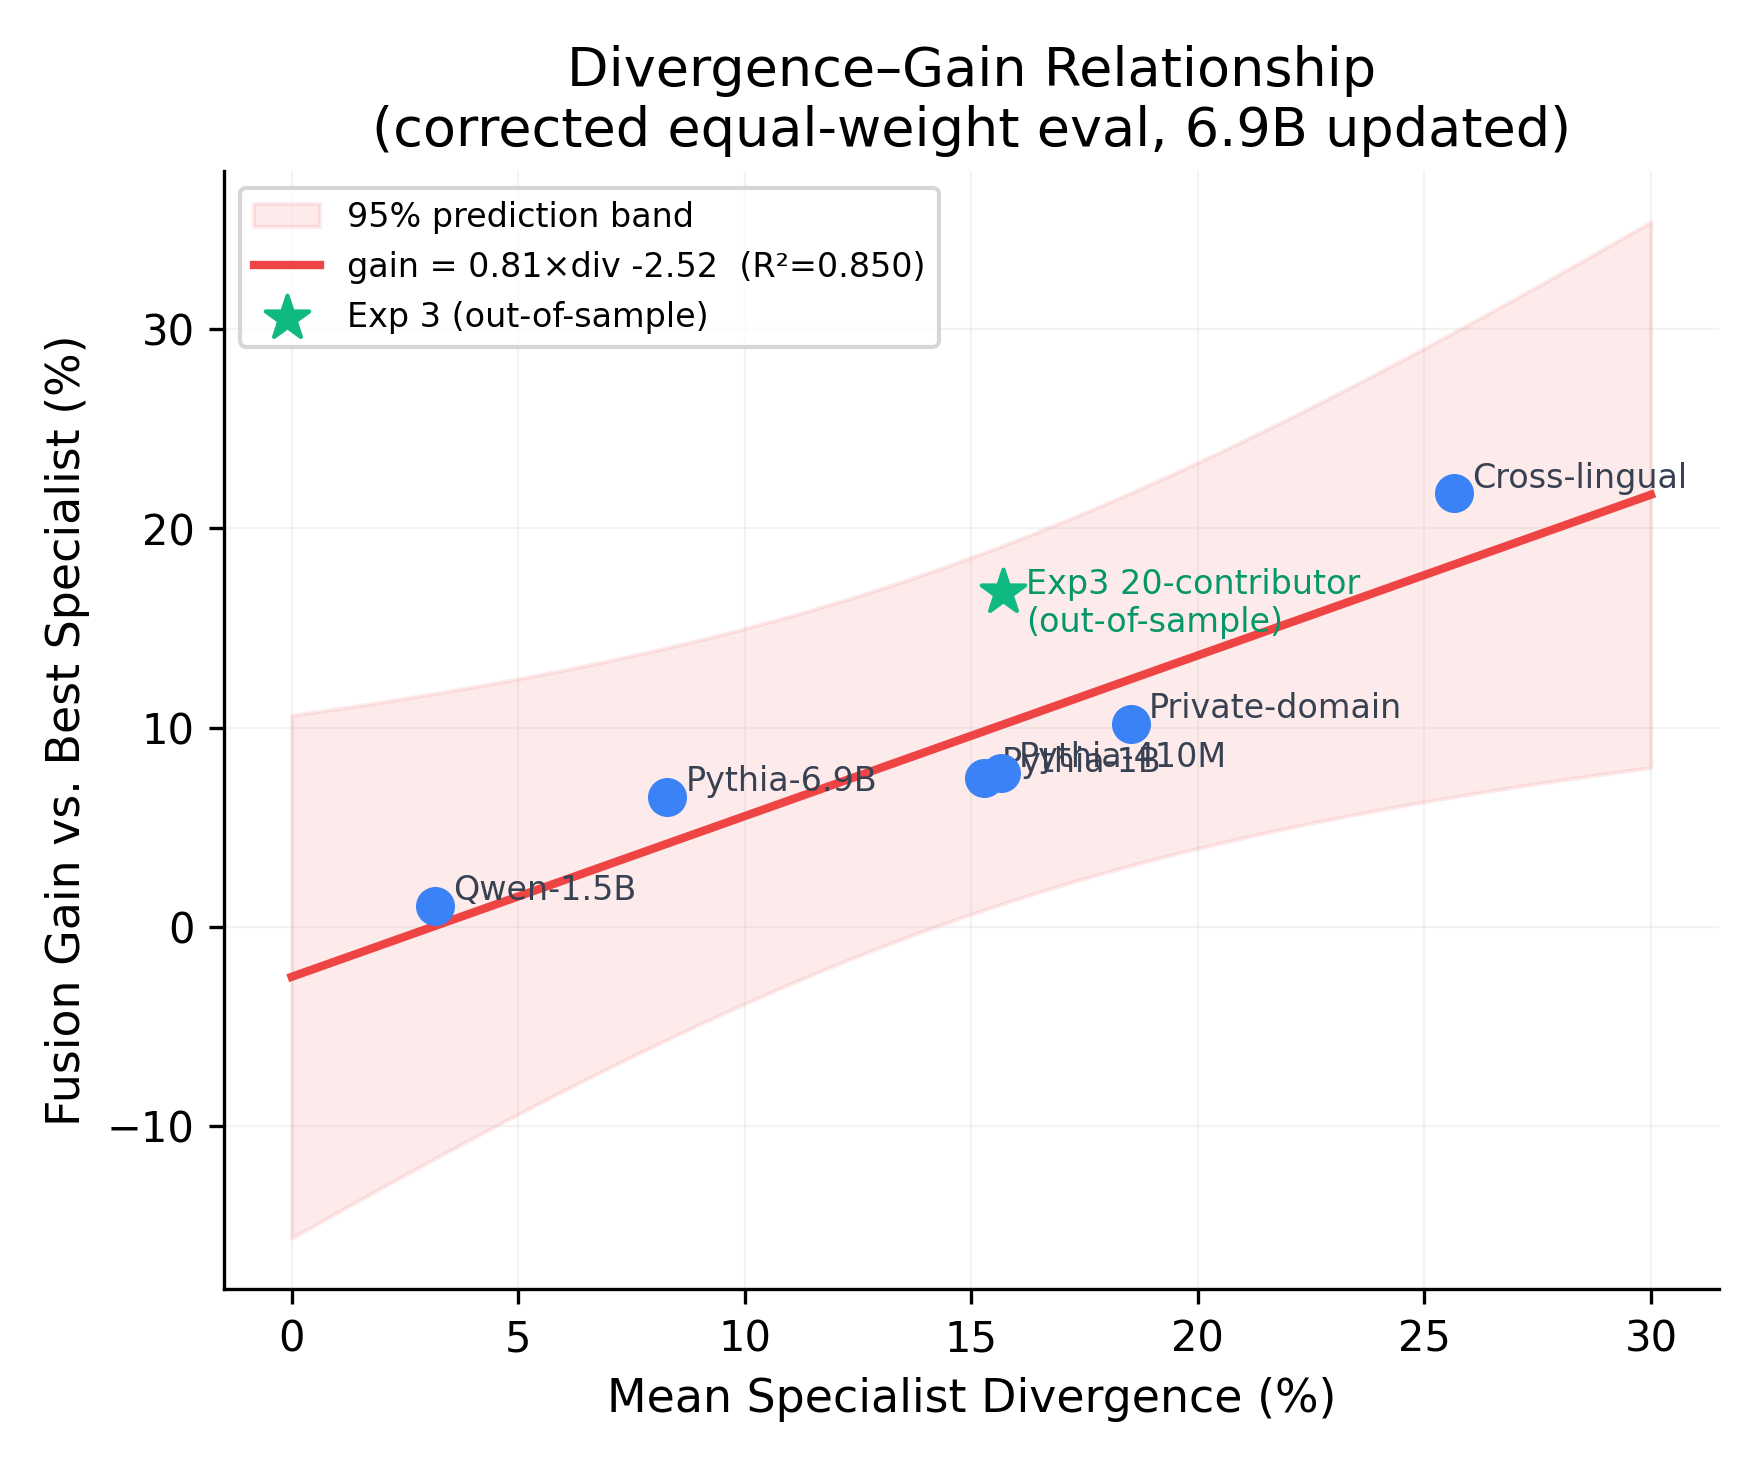
\includegraphics[width=0.82\textwidth]{fig_divergence_gain_regression}
  \caption{Fusion gain vs.\ mean specialist divergence (\%) with OLS regression line and 95\% prediction band. Linear fit: $\text{gain} = -2.72 + 0.82 \times \text{div}$ ($R^2 = 0.856$, $n=6$ in-sample conditions). English-domain conditions cluster near the line; Exp 2 (private, purple) and Exp 1 (cross-lingual, red) lie above prediction, consistent with base-model incompetence producing outsized gains (+3.6pp for cross-lingual). Exp~3 (20-contributor, 15.68\%, +16.71\%) is an out-of-sample validation point (+6.57pp above regression).}
  \label{fig:divergence_gain_regression}
\end{figure}

\section{Base-Model Competence as Secondary Predictor}
\label{app:baseppl}

Across the six experimental conditions, log base-model perplexity correlates with conversion efficiency (gain / divergence) at $r = +0.560$ (Pearson, $n = 6$; linear scale: $r = +0.545$). For comparison, specialist divergence correlates with conversion efficiency at $r = +0.614$. On the six-point sample these are suggestive rather than definitive, but mechanistically plausible: when the base model achieves near-random perplexity (Yoruba PPL $\approx 42$), the specialist corrects from a high-loss floor and the router routes with near-certainty. When the base is already competent (English code PPL $\approx 7$), gains are smaller. A two-factor heuristic---measure both specialist divergence and base-model competence before committing to a cooperative---may help practitioners assess expected gains.

\begin{figure}[h]
  \centering
  
\includegraphics[width=\linewidth]{figures/paper/fig_baseppl_conversion.png}
  \caption{Base-model perplexity as a secondary predictor of cooperative fusion efficiency. \textbf{Left}: Conversion efficiency (gain/div) vs.\ mean base-model perplexity (linear scale, $r=+0.545$). \textbf{Centre}: Same with log-scaled perplexity axis ($r=+0.560$). \textbf{Right}: Conversion efficiency vs.\ specialist divergence ($r=+0.614$). $n=6$ conditions.}
  \label{fig:baseppl_conversion}
\end{figure}

\end{document}
